%\documentclass[letter,mathserif,usenames,dvipsnames,aspectratio=169]{gkibeamer}
\documentclass[letter,mathserif,usenames,dvipsnames]{gkibeamer}

%% note: use this for handout mode!
%\documentclass[mathserif,handout,4-on-1]{gkibeamer}


%% note: use this for handout mode!
%%\documentclass[mathserif,handout,4-on-1]{gkibeamer}

\usepackage{amsmath,amssymb,amsthm}
\usepackage{nicefrac}
\usepackage{array}
\usepackage{xspace}
\usepackage{multirow}
%\usepackage{realboxes}
%\usepackage{algorithmic}

\usepackage{media9}

\usepackage{graphicx}
\usepackage{booktabs}
\usepackage{enumerate}
\usepackage[absolute,overlay]{textpos}
\usepackage{pifont}

\usepackage{tikz}
\usetikzlibrary{shapes,positioning,calc,intersections}
\usetikzlibrary{tikzmark,fit,shapes.geometric}
\usetikzlibrary{arrows}
\newcommand{\TargetVariable}[1]{\underline{#1}}
%\usetikzlibrary{arrows,petri,automata,snakes}

\tikzstyle{every transition}=[minimum size=4mm]
\tikzstyle{every place}=[minimum size=4mm]
\tikzstyle{pnplace}=[shape=circle,place,thick,inner sep=0.05mm]
\tikzstyle{pntrans}=[transition,thick,inner sep=0.5mm]

\pgfmathsetseed{\pdfuniformdeviate 10000000} % new seed at each compilation

\usepackage{framedboxes}

\definecolor{lightskyblue}{cmyk}{0.31,0.11,0.0,0.0}
\newcommand{\hilite}{\textcolor{structure}}

\newcommand{\Omit}[1]{}
\newcommand{\NoOmit}[1]{#1}
\newcommand{\tup}[1]{\langle #1 \rangle}
\newcommand{\denselist}{\itemsep 0pt \topsep 0pt}
\newcommand{\sci}[2]{#1\textsc{e}#2}

\newcommand{\TBD}[1]{\textbf{TBD:} #1}

\newcommand{\red}[1]{\textcolor{Red}{#1}}
\newcommand{\green}[1]{\textcolor{OliveGreen}{#1}}

%\usepackage[table]{xcolor}
\usepackage{colortbl}
\newcommand{\G}{\cellcolor[gray]{0.75}}

\renewcommand{\P}{\mathbb{P}}
\newcommand{\R}{\mathcal{R}}


\usepackage{relsize}
\newcommand{\join}{\mathlarger{\Join}}
\DeclareMathOperator{\bigjoin}{\mathlarger{\mathlarger{\mathlarger{\Join}}}}

%% Set bold frame titles
\setbeamerfont{frametitle}{series=\bfseries\centering}

%% This makes invisible the covered items
\setbeamercovered{transparent}

%% This makes the text in second-/third-level lists same font size as
%% in first-level lists
\setbeamerfont{itemize/enumerate subbody}{size=\normalsize}
\setbeamerfont{itemize/enumerate subsubbody}{size=\normalsize}
\setbeamerfont{itemize/enumerate subitem projected}{size=\normalsize}
\setbeamerfont{itemize/enumerate subsubitem projected}{size=\normalsize}

%% This makes the bullets in second/third level list same size as
%% in first-level lists
\makeatletter
%\setbeamertemplate{itemize subitem}{\beamer@usesphere{subitem projected}{bigsphere}}
%\setbeamertemplate{itemize subsubitem}{\beamer@usesphere{subsubitem projected}{bigsphere}}
\setbeamertemplate{itemize subitem}{\tiny\raise1.5pt\hbox{\donotcoloroutermaths$\blacktriangleright$}}
%\setbeamercolor{itemize item}{fg=OliveGreen}
%\setbeamercolor{enumerate item}{fg=OliveGreen}
\setbeamercolor{itemize item}{fg=black}
\setbeamercolor{enumerate item}{fg=black}
%\setbeamercolor{itemize subitem}{fg=OliveGreen}
%\setbeamercolor{itemize subsubitem}{fg=default}
\makeatother

%% Reduces list indentation and label space
\setlength{\leftmargini}{1em}
\setlength{\leftmarginii}{0.75em}
\setlength{\leftmarginiii}{0.75em}
\setlength{\labelsep}{.5em}
\setlength{\labelwidth}{1em}

\setbeamersize{text margin left=0.75cm, text margin right=0.75cm}

%% this changes the margins on the hand-out version (I think it is
%% to make it more similar to the slides version).
\mode<handout>{%
  \setbeamersize{text margin left=0.75cm}
  \setbeamersize{text margin right=1.75cm}
}

\newcommand{\naturals}{\ensuremath{\mathbb{N}}}
\newcommand{\reals}{\ensuremath{\mathbb{R}}}
\newcommand{\indicator}[1]{[\![#1]\!]}

\newcommand<>{\textblue}[1]{{\color#2{blue}#1}}
\newcommand<>{\textbg}[1]{{\color#2{bg}#1}}

\newcommand<>{\gray}[1]{\textcolor#2{gray}{#1}}
\newenvironment<>{grayenv}{\color#1{gray}}{}

%\newcommand{\Alert}[1]{\alert{\bf #1}}
\newcommand{\Alert}[1]{\textcolor{blue!70!black}{\bf #1}}
\newcommand{\AlertSecondary}[1]{\textcolor{blue!70!black}{#1}}
\newcommand{\RedAlert}[1]{\textcolor{red}{\bf #1}}

\definecolor{customblue}{rgb}{0.129216,0.188235,0.709804}


%\setbeamertemplate{blocks}[framed]
%\setbeamercolor{block title}{fg=darkblue!80!yellow, bg=gray!30}%white!80!yellow!85!orange}
%\setbeamercolor{block title}{fg=black, bg=gray!40}%white!80!yellow!85!orange}
%\setbeamercolor{block body}{fg=darkblue!80!yellow, bg=gray!20}%yellow!20!orange}
%\setbeamercolor{block body}{fg=black, bg=gray!20}%yellow!20!orange}
\setbeamerfont{block title}{series=\bfseries}
\setbeamerfont{block body}{series=\itshape}
\setbeamercolor{block title}{fg=white, bg=customblue!100}
\setbeamercolor{block body}{fg=black, bg=customblue!5}
\setbeamercolor{postit}{bg=yellow!50!white}


\newcommand{\SAS}{\ensuremath{\text{SAS}^+}\xspace}
\newcommand{\hplus}{\ensuremath{h^+}\xspace}
\newcommand{\hlmcut}{\ensuremath{h^{\text{LM-cut}}}\xspace}
\newcommand{\myhlmcut}{\ensuremath{h^{\text{LM-cut}}_{\text{ours}}}\xspace}
\newcommand{\hla}{\ensuremath{h^{\text{LA}}}\xspace}
\newcommand{\hms}{\ensuremath{h^{\text{M\&S}}}\xspace}
\newcommand{\HSPf}{\ensuremath{\text{HSP}^*_F}\xspace}
\newcommand{\hseq}{\ensuremath{h^{\text{SEQ}}}\xspace}
\newcommand{\hiseq}{\ensuremath{h^{\text{iSEQ}}}\xspace}
\newcommand{\hseqsafe}{\ensuremath{h^{\text{SEQ}}_\text{safe}}\xspace}
\newcommand{\hm}{\ensuremath{h^m}\xspace}

\newcommand{\pit}[1]{\text{pit@$#1$}}
\newcommand{\breeze}[1]{\text{breeze@$#1$}}
\newcommand{\map}[1]{\text{cell@$#1$}}
\newcommand{\sensor}[1]{\text{sensed@$#1$}}

\newcommand{\ellipse}[4]{
  \visible<#1>{
  \begin{tikzpicture}[remember picture,overlay]
  \coordinate[draw,line width=.75pt,blue!70!black,ellipse,inner xsep=#2, inner ysep=#3,fit={(pic cs:#4)}] {};
  \end{tikzpicture}
  }
}

\newcommand{\mymark}[1]{\raisebox{3pt}{\tikzmark{#1}}}

\newcommand{\widthofbold}[1]{%
\settowidth{\dimen0}{\textbf{#1}}%
\makebox[\dimen0]{#1}}
\newcommand<>{\bold}[1]{%
\alt#2{\textbf{#1}}{\widthofbold{#1}}}
\makeatother

\mode<beamer>{
  \title{\bf Algoritmos para Juegos con Informaci\'on\\Incompleta y No Determinismo}
  \author{Rubmary Rojas}
  \institute{Universidad Sim\'on Bol\'{\i}var, Caracas, Venezuela}
  \date{Enero 2020}
}

% Only if sectionpage is undefined
%\newcommand{\sectionpage}{}

\definecolor{c231f20}{RGB}{35,31,32}
\newcommand{\logousb}[1][0.0333]{%
\begin{tikzpicture}[y=0.80pt,x=0.80pt,yscale=-1, inner sep=0pt, outer sep=0pt]
\begin{scope}[cm={{1.25,0.0,0.0,-1.25,(0.0,142.5)}}]
  \begin{scope}[scale=#1]
    \path[fill=c231f20,even odd rule] (852.7580,526.1290) -- (779.6020,496.6410) --
      (777.0080,504.4880) -- (556.5040,415.5860) .. controls (550.8120,413.5230) and
      (547.0160,408.1170) .. (547.0160,402.0700) -- (547.0160,53.4688) --
      (555.6760,48.5000) -- (555.6760,3.0898) -- (497.4920,3.0391) --
      (497.4920,75.9414) -- (504.9220,73.9492) -- (504.9220,401.8010) .. controls
      (504.9220,427.0270) and (521.9060,449.1090) .. (546.3120,455.6370) --
      (763.9840,543.8480) -- (761.1170,552.5000) -- (852.7580,589.4410) --
      (944.6330,551.4100) -- (941.8320,543.0000) -- (1158.5000,454.2230) .. controls
      (1181.5200,446.1020) and (1200.6000,432.7580) .. (1200.6000,400.5550) --
      (1199.3600,68.9453) -- (1206.8300,72.3359) -- (1206.8300,0.6445) --
      (1148.6400,0.6445) -- (1148.6400,45.2930) -- (1157.3200,49.6680) --
      (1158.5000,402.0510) .. controls (1158.5000,408.1050) and (1151.7200,413.3090)
      .. (1146.0300,415.3710) -- (928.5080,504.4690) -- (925.9140,496.6250) --
      (852.7580,526.1290);
    \path[fill=c231f20,even odd rule] (852.7580,414.3950) -- (811.9140,397.9800) --
      (809.1840,407.2420) -- (648.5160,342.4650) -- (648.5160,19.2695) --
      (657.1760,15.2930) -- (657.1760,2.9414) -- (599.0000,3.1367) --
      (599.0000,31.5977) -- (606.4260,31.4023) -- (606.4260,370.9570) --
      (795.9100,447.3590) -- (793.1990,455.5470) -- (852.7580,479.5040) --
      (912.2070,454.0470) -- (909.7230,446.5980) -- (1097.8500,368.4490) --
      (1097.8500,29.8320) -- (1104.0000,29.0625) -- (1104.0000,0.6445) --
      (1045.8500,0.6445) -- (1045.8500,13.9688) -- (1055.7600,18.5898) --
      (1055.7600,340.6520) -- (896.3550,406.4530) -- (893.5080,397.9060) --
      (852.7580,414.3950);
    \path[fill=c231f20,even odd rule] (852.7580,697.0160) -- (729.7110,647.4180) --
      (732.2030,639.8750) -- (493.0780,543.4410) .. controls (438.4020,517.9960) and
      (403.4260,463.1990) .. (403.4260,402.9800) -- (403.4260,136.7810) --
      (395.9880,141.3520) -- (395.9880,9.6445) .. controls (415.2380,6.7813) and
      (434.8750,5.0391) .. (454.2380,4.5938) -- (454.1800,102.7770) --
      (444.2770,109.7420) -- (444.2770,406.9840) .. controls (444.2770,407.0390) and
      (444.2770,407.0940) .. (444.2770,407.1410) .. controls (444.2770,448.5430) and
      (468.3200,486.2110) .. (505.9100,503.7030) -- (745.0390,601.0980) --
      (748.0080,592.1290) -- (852.7580,634.3670) -- (957.9880,591.5040) --
      (961.0900,600.8160) -- (1199.3600,502.6600) .. controls (1235.5100,482.3050)
      and (1258.9500,449.6520) .. (1261.2400,407.1090) .. controls
      (1261.2500,407.0590) and (1261.2400,407.0040) .. (1261.2400,406.9530) --
      (1259.6700,105.1250) -- (1250.1800,97.8828) -- (1249.4200,0.6445) .. controls
      (1268.7800,1.0937) and (1288.8500,3.0312) .. (1308.1000,5.8945) --
      (1308.5300,136.1720) -- (1302.1000,133.0310) -- (1303.1000,409.4060) ..
      controls (1302.1000,464.4800) and (1265.9600,516.8090) .. (1212.7200,541.9730)
      -- (974.1290,638.5940) -- (976.5200,647.1480) -- (852.7580,697.0160);
    \path[fill=c231f20,even odd rule] (892.3670,0.6445) -- (892.3670,232.3200) --
      (852.7580,249.5900) -- (811.9140,233.1250) -- (811.9140,0.6445) --
      (892.3670,0.6445);
    \path[fill=c231f20,even odd rule] (852.7580,315.7420) -- (953.0230,273.8870) --
      (953.0230,0.6445) -- (993.8710,0.6445) -- (993.8710,301.2850) --
      (878.3870,348.4920) -- (878.5860,358.0000) -- (852.7580,368.4880) --
      (824.8750,357.2460) -- (826.8710,348.7540) -- (710.4100,301.7930) --
      (710.4100,0.6445) -- (750.0270,0.6445) -- (750.0270,274.3200) --
      (852.7580,315.7420);
    \path[fill=c231f20,even odd rule] (852.7580,742.9650) -- (716.2970,687.9610) --
      (713.5860,696.1410) -- (468.3240,596.7540) .. controls (392.3790,561.4140) and
      (343.8050,485.3090) .. (343.8050,401.6680) -- (343.8050,176.9450) --
      (353.9060,169.5860) -- (353.9180,17.9219) .. controls (333.3830,23.0156) and
      (312.9570,29.5859) .. (293.2580,37.3828) -- (293.2540,209.1560) --
      (301.9180,205.1760) -- (301.9180,399.7460) .. controls (301.9180,506.4300) and
      (366.8360,602.4690) .. (465.9260,642.4530) -- (700.0660,737.0080) --
      (697.5740,744.5430) -- (852.7580,807.1020) -- (1008.6400,743.5860) --
      (1006.1200,736.0230) -- (1245.9500,638.0980) .. controls (1345.0400,595.3320)
      and (1404.8400,506.3980) .. (1404.8400,399.7150) -- (1404.8400,200.3830) --
      (1413.1600,203.3550) -- (1411.0700,33.7734) .. controls (1391.3600,25.9805)
      and (1372.2300,19.2070) .. (1351.7000,14.1211) -- (1352.9000,164.8870) --
      (1361.5200,170.6520) -- (1363.9100,401.6370) .. controls (1359.9200,485.2810)
      and (1312.1400,563.3750) .. (1235.7900,596.3280) -- (992.5270,695.2110) --
      (989.9450,687.4530) -- (852.7580,742.9650);
    \path[fill=c231f20,even odd rule] (852.7580,853.3010) -- (684.0860,785.2930) --
      (681.3440,793.5820) -- (436.9180,693.0080) .. controls (353.9060,656.7150) and
      (252.4100,584.7700) .. (242.5000,398.4730) -- (242.5000,243.5820) --
      (252.4100,236.4960) -- (251.0310,59.4492) .. controls (226.6800,67.7656) and
      (208.3520,80.8984) .. (191.7540,94.7852) -- (191.7540,275.5120) --
      (202.0040,271.2540) -- (201.6760,371.8440) .. controls (201.6410,600.1680) and
      (326.5660,699.0390) .. (444.2770,741.1880) -- (668.4140,832.6640) --
      (665.8050,840.5510) -- (853.4730,916.4570) -- (1040.6800,839.7970) --
      (1038.0800,831.9730) -- (1286.2200,730.5270) .. controls (1358.3900,703.7770)
      and (1492.0000,608.8440) .. (1506.3400,414.5620) -- (1506.4100,266.1170) --
      (1516.2600,269.3010) -- (1513.8100,89.7227) .. controls (1499.7900,79.7656)
      and (1478.6100,63.3203) .. (1454.1300,52.5352) -- (1455.6300,232.4450) --
      (1465.4900,239.8120) -- (1465.4900,412.2230) .. controls (1459.6800,482.1090)
      and (1432.3800,625.0660) .. (1266.0200,694.7620) -- (1025.1500,793.1410) --
      (1022.3300,784.6800) -- (852.7580,853.3010);
    \path[fill=c231f20,even odd rule] (853.9490,961.2930) -- (652.6990,880.1520) --
      (648.5160,888.3710) -- (396.4960,784.6050) .. controls (287.1450,741.4380) and
      (154.4220,611.9100) .. (144.4840,416.4140) -- (143.4730,309.9220) --
      (152.1290,303.2500) -- (149.6800,132.0080) .. controls (120.3090,155.2970) and
      (104.9180,175.3280) .. (90.2500,195.8200) -- (91.4805,343.6640) --
      (100.1480,338.1800) -- (101.7500,410.5740) .. controls (108.6680,640.3670) and
      (253.2770,772.3440) .. (395.9880,830.3910) -- (636.3790,929.4800) --
      (633.7230,937.5040) -- (852.7580,1025.8200) -- (1072.0700,937.2970) --
      (1070.1600,928.3050) -- (1302.1000,833.1090) .. controls (1404.8400,797.4490)
      and (1594.7100,667.6480) .. (1606.6100,427.7540) -- (1606.6100,334.3360) --
      (1615.8200,339.1480) -- (1615.8000,191.4920) .. controls (1606.6100,177.9060)
      and (1584.3200,147.6950) .. (1555.6600,123.9610) -- (1557.1100,299.4220) --
      (1565.7600,305.9410) -- (1564.4600,422.1170) .. controls (1555.5600,568.6880)
      and (1469.2200,729.0200) .. (1268.7600,802.0980) -- (1057.2600,889.5740) --
      (1053.9800,879.7110) -- (853.9490,961.2930);
    \path[fill=c231f20,even odd rule] (41.9688,376.5660) -- (44.2852,453.1520) ..
      controls (87.2461,748.5270) and (306.2620,865.1170) .. (398.9100,895.0980) --
      (617.9960,985.0350) -- (620.4920,977.4880) -- (853.5310,1071.2900) --
      (1086.3000,976.7580) -- (1088.8000,984.2620) -- (1270.5700,910.7770) ..
      controls (1588.8000,802.2770) and (1658.3700,560.4340) .. (1667.3000,413.5820)
      -- (1667.2600,373.8160) -- (1658.2300,366.0310) -- (1658.6400,268.1450) ..
      controls (1701.8300,340.0700) and (1704.3900,443.0510) .. (1704.3900,468.3550)
      .. controls (1659.5900,794.6640) and (1398.8400,908.6640) ..
      (1303.9100,941.7890) -- (1101.9800,1023.8400) -- (1104.8100,1032.3300) --
      (854.5700,1134.5000) -- (602.2230,1032.7000) -- (604.9450,1024.4600) --
      (397.8010,939.0660) .. controls (182.3950,864.6250) and (29.4805,693.5310) ..
      (3.6055,464.6600) .. controls (3.6055,399.6560) and (17.4492,335.2930) ..
      (44.0469,276.0350) .. controls (45.4023,273.3550) and (47.1836,271.5230) ..
      (49.3633,270.4920) -- (49.3633,370.8010) -- (41.9688,376.5660);
  \end{scope}
\end{scope}

\end{tikzpicture}
}

\begin{document}
\begin{frame}
\maketitle
\begin{center}
    \logousb
\end{center}
\end{frame}

\begin{frame}{\Large Agenda}
\begin{enumerate}
\item Teor\'ia de juegos.
\item Juegos en forma normal:
\begin{itemize}
  \item Modelo y estrategias.
  \item Equilibrio de Nash.
  \item Regret Matching: algoritmo, experimentos y conclusiones.
\end{itemize}
\item Juegos en forma extensiva:
\begin{itemize}
  \item Modelo y estrategias.
  \item Kuhn Poker.
  \item Counterfactual Regret Minimization (CFR): algoritmo, experimentos y conclusiones.
\end{itemize}
\item Conclusiones y Recomendaciones.
\item Demo.
\end{enumerate}
\end{frame}

\begin{frame}{\Large Teor\'ia de Juegos}
\begin{block}{Definici\'on}
  \begin{itemize}
    \item Estudio de \textbf{modelos matem\'aticos} de \textbf{conflicto} y \textbf{cooperaci\'on}.
    \item Agentes que toman decisiones de forma \textbf{racional} e \textbf{inteligente}.
  \end{itemize}
\end{block}
\vspace{.5cm}
\Alert{Aplicaciones}
\begin{center}
\begin{tabular}{@{}cccc@{}}
  
\includegraphics[height=.15\textwidth]{../images/ciencias_sociales.png} &
  
\includegraphics[height=.15\textwidth]{../images/economia.png} &
  
\includegraphics[height=.15\textwidth]{../images/matematica.png} &
  
\includegraphics[height=.15\textwidth]{../images/computacion.png} \\
  & & & \\
  \textbf{Ciencias sociales} &
  \textbf{Econom\'ia} &
  \textbf{Matem\'atica} &
  \textbf{Computaci\'on} \\
\end{tabular}
\end{center}
\end{frame}

\newsavebox{\picbox}
\newcommand{\cutpic}[3]{
\savebox{\picbox}{\includegraphics[height=#2]{#3}}
\tikz\node [draw, rounded corners=#1, line width=4pt,
color=white, minimum width=1.1\wd\picbox,
minimum height=1.1\ht\picbox, path picture={
  \node at (path picture bounding box.center) {
    \usebox{\picbox}};
}] {};}

\begin{frame}{\Large Juegos no deterministas \\ con informaci\'on incompleta}

\begin{columns}
\column{.45\textwidth}
\begin{center}
\begin{block}{No determinismo}
Incertidumbre probabil\'istica: \\
- Lanzar dados \\
- Repartir cartas
\end{block}
{\cutpic{5mm}{.32\textwidth}{../images/dados.jpg}}
\end{center}

\column{.45\textwidth}
\begin{center}
\begin{block}{Informaci\'on incompleta}
Informaci\'on parcial sobre algunas de las acciones que fueron tomadas previamente.%
\end{block}
{\cutpic{5mm}{.32\textwidth}{../images/poker.jpg}}
\end{center}
\end{columns}

\vspace{.5cm}
\Alert{Interrogantes}
\begin{enumerate}[--]
  \item ?`Qu\'e significa que un juego sea resuelto?
  \item ?`Cu\'ando un jugador juega de forma \'optima?
\end{enumerate}
\end{frame}

\begin{frame}{\Large Objetivo General}%\Large Objetivos}
%\begin{block}{Objetivo General}
\centering{Comprender los conceptos en el \'area de juegos de dos personas que involucran informaci\'on incompleta y no determinismo, as\'i como implementar los algoritmos para resolverlos, realizando experimentos sobre distintos juegos que son capturados por el modelo.}
%\end{block}
% \begin{itemize}
%   \visible<2->{\onslide<2>{\item Comprender los diferentes modelos de juegos.}}
%   \visible<3->{\onslide<3>{\item Comprender diferentes conceptos de soluci\'on.}}
%   \visible<4->{\onslide<4>{\item Comprender los resultados te\'oricos m\'as relevantes.}}
%   \visible<5->{\onslide<5>{\item Implementar los algoritmos de Regret Matching y Counterfactual Regret Minimization.}}
%   \visible<6->{\onslide<6>{\item Implementar clases que permitan representar los juegos.}}
%   \visible<7->{\onslide<7>{\item Realizar experimentos sobre los juegos propuestos.}}
%   \visible<8->{\onslide<8>{\item Evaluar las estrategias obtenidas.}}
% \end{itemize}
\end{frame}

\begin{frame}
  \centering{\resizebox{!}{.5cm}{\Alert{Forma Normal o Estrat\'egica}}}
\end{frame}

\begin{frame}{\Large Juegos en Forma Normal o Estrat\'egica}

\Alert{Piedra, papel o tijera}
\vspace{.5cm}

\begin{tabular}{l |c | c | c | l }
\multicolumn{1}{c}{} &  \multicolumn{1}{c}{ $\mathcal{R}$ \raisebox{3pt}{\tikzmark{sp2}}(piedra)} & \multicolumn{1}{c}{$\mathcal{P}$ (papel)} & \multicolumn{1}{c}{$\mathcal{S}$ (ti\raisebox{3pt}{\tikzmark{ep2}}jera)} & \ \
\visible<3>{\textcolor{blue!70!black}{jugador 2}} \\ \cline{2-4}
$\mathcal{R}$ (piedra) & $0,0$ & $-1,1$ & $1,-1$ & \visible<7->{\multirow{3}{*}{\shortstack{Juego de \\ dos jugadores\\de suma cero}}} \\ \cline{2-4}
$\mathcal{P}$ (p\raisebox{3pt}{\tikzmark{p1}}apel)  & $1,-1$ & $0,0$ & $-1,1$ & \\ \cline{2-4}
$\mathcal{S}$ (tijera) & $-1,1$ & $1,$\raisebox{3pt}{\tikzmark{u}}$-1$ & $0,0$ & \\ \cline{2-4}
\multicolumn{1}{c}{} &
  \multicolumn{3}{c}{
    \only<4>{\small{primer jugador \textbf{gana} 1}}
    \only<5>{\small{segundo jugador \textbf{pierde} 1}}
  }
 & \multicolumn{1}{c}{}\\
\multicolumn{2}{l}{\visible<2>{\textcolor{blue!70!black}{jugador 1}}} &
\multicolumn{3}{c}{}
\end{tabular}

\vspace{.5cm}
\begin{columns}[t]
\column{.45\textwidth}
\visible<6->{
\Alert{Elementos}
\begin{enumerate}
  \item Jugadores.
  \item Acciones o estrategias puras: $\mathcal{R}$, $\mathcal{P}$, $\mathcal{S}$.
  \item Funci\'on de pago o utilidades.
\end{enumerate}
}
\column{.52\textwidth}
\visible<8->{
\Alert{Estrategias}
\begin{enumerate}
  \item Estrategias puras: siempre se elige la misma acci\'on.
  \item Estrategias mixtas: cada acci\'on se elige con cierta probabilidad.
\end{enumerate}
}
\end{columns}

\visible<2>{
\begin{tikzpicture}[remember picture,overlay]
\coordinate[draw,line width=.75pt,blue!70!black,ellipse, inner xsep=22pt, inner ysep=24pt, fit={(pic cs:p1)}] {};
\end{tikzpicture}
}
\visible<3>{
\begin{tikzpicture}[remember picture,overlay]
\coordinate[draw,line width=.75pt,blue!70!black,ellipse,inner ysep=7pt,fit={(pic cs:sp2) (pic cs:ep2)}] {};
\end{tikzpicture}
}
\visible<4-5>{
\begin{tikzpicture}[remember picture,overlay]
\coordinate[draw,line width=.75pt,blue!70!black,ellipse,inner xsep=15, inner ysep=5pt,fit={(pic cs:u)}] {};
\end{tikzpicture}
}
\end{frame}

\begin{frame}{\Large Juegos en Forma Normal o Estrat\'egica}

\Alert{Batalla de los sexos}
\vspace{.5cm}

\begin{columns}
\column{.7\textwidth}
\begin{tabular}{ c c | c | c |}

& \multicolumn{1}{c}{} & \multicolumn{2}{c}{\AlertSecondary{Jos\'e}} \\
& \multicolumn{1}{c}{} &
\multicolumn{1}{c}{\quad\ ballet \quad\quad} &
\multicolumn{1}{c}{\quad\,b\'eisbol \quad\quad}  \\ \cline{3-4}

\multirow{2}{*}{\AlertSecondary{Mar\'ia}}
& ballet    &
  \ \ \onslide<1-11, 13->{$2$}\onslide<1-10, 13->{$,\,$}\mymark{ballet}\onslide<1-10, 12->{$1$} \mymark{elegirBallet}&
  \onslide<1-10, 13->{$0,\,$}\mymark{differentsA}\onslide<1-10, 12->{$0$} \\ \cline{3-4}
& b\'eisbol &
  \onslide<1-11, 13->{$0$}\onslide<1-10, 13->{$,\,$\mymark{differentsB}$0$} &
  \onslide<1-10, 13->{$1$\mymark{beisbol}$,2$} \\ \cline{3-4}

\end{tabular}
\ellipse{2}{12pt}{5pt}{differentsA}
\ellipse{2}{12pt}{5pt}{differentsB}
\ellipse{3,8,10-13}{12pt}{5pt}{ballet}
\ellipse{4,10,13}{12pt}{5pt}{beisbol}
\ellipse{7}{2.5cm}{7pt}{elegirBallet}

\column{.3\textwidth}%
\only<2>{Ninguno obtiene ganancia.}%
\only<3>{Mar\'ia obtiene una ganancia mayor que Jos\'e.}%
\only<4>{Jos\'e obtiene una ganancia mayor que Mar\'ia.}%
\only<7>{Si Mar\'ia siempre elige ballet.}%
\only<8>{Lo mejor para Jos\'e es siempre elegir ballet.}%
\only<11>{Mar\'ia no tiene motivos para cambiar su estrategia.}%
\only<12>{Jos\'e no tiene motivos para cambiar su estrategia.}%
\only<15->{%
  {Lanzar una moneda
  \begin{enumerate}
  \item cara $\implies$ ballet
  \item sello $\implies$ b\'eisbol
  \end{enumerate}}}
\end{columns}

\vspace{.8cm}

\begin{columns}
\column{.4\textwidth}
\visible<5->{
\Alert{Conceptos}
\begin{enumerate}
  \visible<5->{\onslide<5>{\item Ganancia Esperada}}
  \visible<6->{\onslide<6-8>{\item Mejor Respuesta}}
  \visible<9->{\onslide<9-13>{\item Equilibrio de Nash}}
  \visible<14->{\onslide<14-15>{\item Equilibrio Correlacionado}}
\end{enumerate}

\column{.5\textwidth}

\only<5>{Valor promedio que un determinado jugador obtendr\'ia si jugara infinitas veces cuando cada jugador utiliza una estrategia dada.}
\only<6-8>{La mejor forma en que puede jugar un jugador dadas las estrategias seleccionadas de sus oponentes.}
\only<9-13>{Cada jugador utiliza una mejor respuesta frente a las estrategias de sus oponentes.}
\only<14->{Puede haber cooperaci\'on entre los jugadores.}
}
\end{columns}
\end{frame}

\begin{frame}{\Large Equilibrio de Nash}

\Alert{Piedra, papel o tijera}
\vspace{.25cm}

\begin{tabular}{l |c | c | c | }
\multicolumn{1}{c}{} &  \multicolumn{1}{c}{ $\mathcal{R}$ (piedra)} & \multicolumn{1}{c}{$\mathcal{P}$ (papel)} & \multicolumn{1}{c}{$\mathcal{S}$ (tijera)} \\ \cline{2-4}
$\mathcal{R}$ (piedra) &
  \onslide<1-2,5,8->{\ 0}\onslide<1-2,8->{,\ 0} &
  \onslide<1-3,8->{-1}\mymark{rp}\onslide<1-2,8->{,\ 1} &
  \onslide<1-2,7->{\ 1}\onslide<1-2,8->{,-1} \\ \cline{2-4}
$\mathcal{P}$ (papel)  &
  \onslide<1-2,5,8->{\ 1}\onslide<1-2,8->{,}\mymark{pr}\onslide<1-2,6,8->{-1} &
  \onslide<1-3,8->{\ 0}\onslide<1-2,8->{,}\onslide<1-2,6,8->{\ 0} &
  \onslide<1-2,7->{-1}\mymark{ps}\onslide<1-2,8->{,}\onslide<1-2,6,8->{\ 1} \\ \cline{2-4}
$\mathcal{S}$ (tijera) &
  \onslide<1-2,5,8->{-1}\mymark{sr}\onslide<1-2,8->{,}\onslide<1-2,4,8->{\ 1} &
  \onslide<1-3,8->{\ 1}\onslide<1-2,8->{,}\onslide<1-2,4,8->{\mymark{sp}-1} &
  \onslide<1-2,7->{\ 0}\onslide<1-2,8>{,}\onslide<1-2,4,8->{\ 0} \\ \cline{2-4}
\end{tabular}

\ellipse{2-3}{15pt}{5pt}{rp}
\ellipse{4}{15pt}{5pt}{sp}
\ellipse{5}{15pt}{5pt}{sr}
\ellipse{6}{15pt}{5pt}{pr}
\ellipse{7}{15pt}{5pt}{ps}

\vspace{.25cm}
\visible<8->{\RedAlert{No todos los juegos tienen un equilibrio de Nash en estrategias puras.}}

\visible<9->{
\vspace{.25cm}
\begin{block}{Teorema de Nash}
Todo juego finito tiene al menos un equilibrio de Nash (en estrategias mixtas).
\end{block}
}

% \visible<10->{
% \vspace{.25cm}
% \Alert{Juegos de Dos Jugadores de Suma Cero}
% \begin{enumerate}[--]
%   \visible<11->{\item Equilibrio de Nash como principal concepto de soluci\'on.}
%   \visible<12->{\item Valor del juego ($u$).}
% \end{enumerate}
% }
\end{frame}

\begin{frame}{\Large Juegos de Dos Jugadores de Suma Cero}
\begin{enumerate}[--]
  \item Equilibrio de Nash como principal concepto de soluci\'on.
  \item Valor del juego ($u$): ganancia del primer jugador cuando ambos jugadores utilizan un equilibrio de Nash.
  \item El juego ``batalla de los sexos'' no cumple estas condiciones.
  % \begin{itemize}
  % \visible<4->{\item El primer jugador garantiza al menos $u$, independientemente de la estrategia de su oponente.}
  % \visible<5->{\item El segundo jugador garantiza al menos $-u$, independientemente de la estrategia de su oponente.}
  % \end{itemize}
\end{enumerate}
\end{frame}

% \begin{frame}{Juegos de Dos Jugadores de Suma Cero}

% \visible<2->{\Alert{Observaciones previas}}
% \begin{enumerate}[--]
%   \visible<3->{\onslide<3,10->{\item En el juego \textbf{batalla de los sexos} los equilibrios de Nash no son soluciones satisfactorias.}}
%   \visible<4->{\onslide<4,10->{\item Diferentes equilibrios de Nash llevan a diferentes ganancias esperadas.}}
% \end{enumerate}

% \vspace{.5cm}
% \visible<5->{\Alert{Equilibrio de Nash en Juegos de Dos Jugadores de Suma Cero}}
% \begin{enumerate}
%   \visible<6->{\onslide<6,10->{\item Soluci\'on satisfactoria.}}
%   \visible<7->{\onslide<7,10->{\item Valor del juego $u$: ganancia esperada del primer jugador cuando ambos jugadores utilizan \textbf{cualquier} equilibrio de Nash.}}
%   \visible<8->{\onslide<8,10->{\item El primer jugador puede garantizar una ganancia esperada de \textbf{al menos} $u$ independientemente de la estrategia de su oponente.}}
%   \visible<9->{\onslide<9,10->{\item El segundo jugador puede garantizar una ganancia esperada de \textbf{al menos} $-u$ independientemente de la estrategia de su oponente.}}
% \end{enumerate}
% \end{frame}

\begin{frame}{\Large Regret Matching: C\'alculo del Equilibrio de Nash}

% \Alert{Algoritmos para calcular un Equilibrio de Nash}
% \begin{itemize}
%   \item Juegos de dos jugadores de suma cero.
% \end{itemize}
\Alert{Esquema General:}
\begin{enumerate}
  \item Se juega de forma repetida a trav\'es del tiempo $t = 1, 2, 3, ...$.
  \item A tiempo $t+1$ cada jugador elige una acci\'on siguiendo una estrategia mixta \textbf{determinada}.
  \item La \textbf{estrategia emp\'irica} converge a un equilibrio de Nash; en la pr\'actica el algoritmo es detenido despu\'es de cierto n\'umero de iteraciones.
\end{enumerate}
\vspace{.25cm}
\visible<2->{%
%\Alert{?`C\'omo calcular la distribuci\'on de probabilidad?}
% \begin{itemize}
%   \item Diferentes formas de calcular la distribuci\'on de probabilidad conducen a diferentes algoritmos.
% \end{itemize}
Diferentes formas de calcular la estrategia mixta conducen a diferentes algoritmos:
\begin{enumerate}
  \item Regret condicional.
  \item Regret incondicional.
  \item Vector invariante de probabilidad.
\end{enumerate}}


% \vspace{.25cm}
% \visible<6->{
% \begin{block}{Regret}
% M\'etrica de \bold<7->{arrepentimiento} de no haber elegido una acci\'on en particular.
% \end{block}
% }
\end{frame}

\begin{frame}{\Large Regret Matching: Procedimientos}
\begin{block}{Regret}
M\'etrica de \textbf{arrepentimiento} de no haber elegido una acci\'on en particular.
\end{block}
\vspace{.6cm}
\begin{columns}
\column{.45\textwidth}
\visible<2->{\Alert{Tres procedimientos}}
\begin{enumerate}
  \visible<2->{\onslide<2-4>{\item Regret condicional.}}
  \visible<5->{\onslide<5-7>{\item Regret incondicional.}}
  \visible<8->{\onslide<8>{\item Vector invariante de probabilidad.}}
\end{enumerate}

\column{.5\textwidth}

\vspace{.3cm}
\visible<2->{%
\begin{tabular}{|p{9mm}p{9mm}p{9mm}|p{5mm}|}
\hline
$\mathcal{R}, \mathcal{S}$ & $\mathcal{R}, \mathcal{P}$ & $\mathcal{S}, \mathcal{S}$ & $\bar{u}$\\ \hline
1 & -1 & 0 & 0\\ \hline
\end{tabular}
}

\vspace{.3cm}
\visible<3-4,6-7>{%
\begin{tabular}{|p{9mm}p{9mm}p{9mm}|p{5mm}|}
\hline
  $\RedAlert{\mathcal{\only<3,6>S\only<4,7->P}}, \mathcal{S}$ &
  $\RedAlert{\mathcal{\only<3,6>S\only<4,7->P}}, \mathcal{P}$ &
  $\only<3-4>{\mathcal{S}}\RedAlert{\only<6>{\mathcal{S}}\only<7->{\mathcal{P}}}, \mathcal{S}$ &
  $\bar{u}$\\ \hline
  \only<3,6>0\only<4,7->{-1}&\only<3,6>1\only<4,7->0&\only<3-4,6>0\only<7->{-1}&\only<4,7->-$\frac{\only<3-4,6>1\only<7->2}{3}$\\ \hline
\end{tabular}
}
\vspace{.3cm}
\visible<3-4, 6-7>{
\begin{tabular}{p{50mm}}
 \only<3>{$R_1(\mathcal{R}, \mathcal{S}\,) = \frac{1}{3} - 0 = \frac{1}{3}$}
 \only<4>{$R_1(\mathcal{R}, \mathcal{P}) = -\frac{1}{3} - 0 = -\frac{1}{3}$}
 \only<6>{$R_1(\mathcal{S}) =  \frac{1}{3} - 0 =  \frac{1}{3}$}
 \only<7->{$R_1(\mathcal{P}) = -\frac{2}{3} - 0 = -\frac{2}{3}$}
\end{tabular}
}
\end{columns}
\end{frame}

\begin{frame}{\Large Regret Matching: Observaciones}
% \Alert{Observaciones}
\begin{enumerate}
  \item Las probabilidades son elegidas proporcional a los regrets positivos.
  \item El regret positivo tiende a cero cuando el n\'umero de juegos tiende a infinito.
  \item Si el regret positivo es peque\~no, la \textbf{estrategia emp\'irica} es una aproximaci\'on a un equilibrio de Nash.
\end{enumerate}
\vspace{.3cm}

\visible<2->{\Alert{Estrategia Emp\'irica}}\\
\vspace{.2cm}
\visible<2->{La probabilidad de que un determinado jugador elija una acci\'on $a$ es igual a:
$$ p(a) = \frac{\text{n\'umero de veces que el jugador eligi\'o }a}{\text{n\'umero total de juegos}}$$}
\end{frame}


% \begin{frame}{\Large Resultados Experimentales}
% \vspace{.5cm}
% \begin{columns}[t]
% \column{.45\textwidth}
% \Alert{Evaluaci\'on y Correctitud}
% \begin{enumerate}
%   \onslide<2,15->{\visible<2->{\item Gr\'aficas del regret incondicional con respecto al n\'umero de iteraciones.}}
%   \onslide<3,15->{\visible<3->{\item Problema equivalente de programaci\'on lineal.}}
%   \visible<4->{\item Explotabilidad\only<14->{: $\varepsilon = \varepsilon_1 + \varepsilon_2$}.}
% \end{enumerate}
% \column{.5\textwidth}
% \visible<5->{%
% \Alert{\only<5-8>{Equilibrio de Nash $\sigma^* = (\sigma^*_1, \sigma^*_2)$}\only<9->{Aproximaci\'on $\sigma' = (\sigma'_1, \sigma'_2)$}}
% \visible<6-8, 10->{%
% \begin{enumerate}
%   \onslide<6,10-11,15->{\visible<6-8, 10->{\item Primer jugador garantiza una ganancia esperada de al menos \only<6-8>{$u$}\only<10->{$u-\varepsilon_1$}.}}
%   \onslide<7-8, 12-13,15->{\visible<7-8, 12->{\item Segundo jugador garantiza una ganancia esperada de \only<7>{al menos $-u$.}\only<8, 12->{a lo sumo} \only<8>{$u$}\only<12->{$u+\varepsilon_2$} \only<8, 12->{para el primer jugador.}}}
% \end{enumerate}}
% }
% \end{columns}
% \begin{center}
%   \begin{tikzpicture}
%   \visible<5->{\draw[<->, very thick] (-5.25, 0) -- (5.25, 0);}
%   \visible<5->{\draw[dashed] (0, 1.5) -- (0, -1.5);}
%   \visible<5->{\node[align=center] at (0.15, 0.2) {\small{$u$}};}
%   \visible<5->{\draw[fill=black] (0, 0) circle (0.05cm);}
%   \visible<6>{\draw[->, rounded corners, blue, very thick](0, 0) -- (0, -0.6) -- (5.25, -0.6);}
%   \visible<6->{\draw[->, rounded corners, blue, very thin](0, 0) -- (0, -0.6) -- (5.25, -0.6);}
%   \visible<6->{\node[text width=3.5cm] at (3.5,-1) {$u_1(\sigma_1^*, \sigma_2) \geq u $};}
%   \only<7>{\node[text width=3.5cm] at (-3,-1) {$u_2(\sigma_1, \sigma^*_2) \geq -u $};}
%   \visible<7->{\draw[->, rounded corners, red, very thin](0, 0) -- (0, -0.5) -- (-5.25, -0.5);}
%   \visible<7-8>{\draw[->, rounded corners, red,  very thick](0, 0) -- (0, -0.5) -- (-5.25, -0.5);}
%   \visible<8->{\node[text width=3.5cm] at (-3,-1) {$u_1(\sigma_1, \sigma^*_2) \leq u $};}
%   \visible<10->{\draw[<->](-0.01, 1) -- (-1.5, 1);}
%   \visible<10->{\draw[dashed] (-1.5, 2) -- (-1.5, -0.45);}
%   \visible<10->{\node[text width=1cm] at (-0.4, 1.25) {$\varepsilon_1$};}
%   \visible<10->{\node[align=left] at (-0.9, 0.2) {\small{$u-\varepsilon_1$}};}
%   \visible<10->{\draw[fill=black] (-1.5, 0) circle (0.05cm);}
%   \visible<11->{\draw[->, rounded corners, blue, very thin](-1.5, 0) -- (-1.5, 0.6) -- (5.25, 0.6);}
%   \visible<11>{\draw[->, rounded corners, blue, very thick](-1.5, 0) -- (-1.5, 0.6) -- ( 5.25, 0.6);}
%   \visible<11->{\node[text width=3.5cm] at (3.5, 1) {$u_1(\sigma'_1, \sigma_2) \geq u - \varepsilon_1$};}
%   \visible<12->{\draw[<->](0.01, 1) -- (0.8, 1);}
%   \visible<12->{\draw[dashed] (0.8, 2) -- (0.8, -0.45);}
%   \visible<12->{\node[text width=1cm] at (0.7, 1.25) {$\varepsilon_2$};}
%   \visible<12->{\node[align=left] at (1.35, 0.2) {\small{$u+\varepsilon_2$}};}
%   \visible<12->{\draw[fill=black] (0.8, 0) circle (0.05cm);}
%   \visible<13->{\draw[->, rounded corners, red, very thin](0.8, 0) -- (0.8, 0.5) -- (-5.25, 0.5);}
%   \visible<13>{\draw[->, rounded corners, red,  very thick]( 0.8, 0) -- ( 0.8, 0.5) -- (-5.25, 0.5);}
%   \visible<13->{\node[text width=3.5cm] at (-3.25, 1) {$u_1(\sigma_1, \sigma'_2) \leq u + \varepsilon_2$};}
%   \visible<14->{\draw[<->](-1.5, 1.7) -- (0.8, 1.7);}
%   \visible<14->{\node[text width=1cm] at (0.1, 2) {$\varepsilon$};}
%   \end{tikzpicture}
% \end{center}
% \end{frame}

\begin{frame}{\Large Regret Matching: Experimentos}

\begin{enumerate}
  \item $4$ juegos para dos jugadores de suma cero.
  \item $10$ corridas por cada uno de los juegos y cada uno de los procedimientos.
  \item Criterio de parada: regret incondicional menor que 0,005.
  \item Gr\'aficas del regret con respecto al n\'umero de iteraciones.
  \item Verificaci\'on realizada con programaci\'on lineal.
  \item Verificaci\'on: la explotabilidad mide la distancia entre la estrategia actual y un equilibrio de Nash.
  % \visible<7->{ \onslide<7->{\item Tabla de resultados:}}%
  % \begin{itemize}%
  %   \visible<8->{ \onslide<8->{\item Ganancia esperada del primer jugador de la \'ultima estrategia obtenida.}}
  %   \visible<9->{ \onslide<9->{\item Explotabilidad de la \'ultima estrategia obtenida.}}
  %   \visible<10->{ \onslide<10->{\item Tiempo promedio.}}
  %   \visible<11->{ \onslide<11->{\item N\'umero de iteraciones promedio.}}
  %   \visible<12->{ \onslide<12->{\item Promedio del tiempo por iteraci\'on.}}
  % \end{itemize}
\end{enumerate}
\end{frame}

\newcommand{\graphicsRM}[1]{
\begin{figure}
    \resizebox{\textwidth}{!}{
    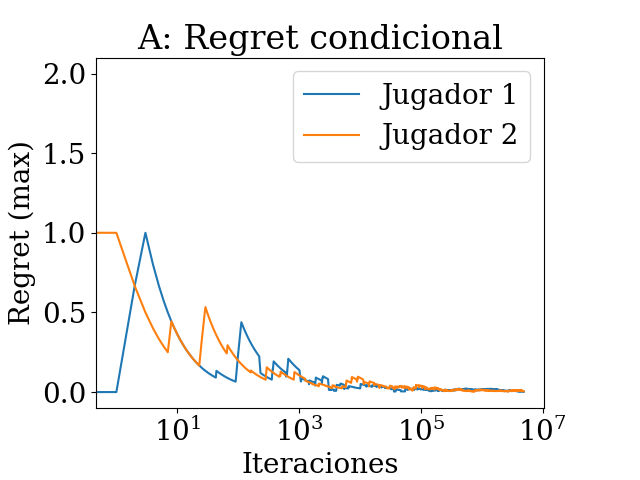
\includegraphics{../graphics/regret-matching/#1/procedimiento-A.png}
    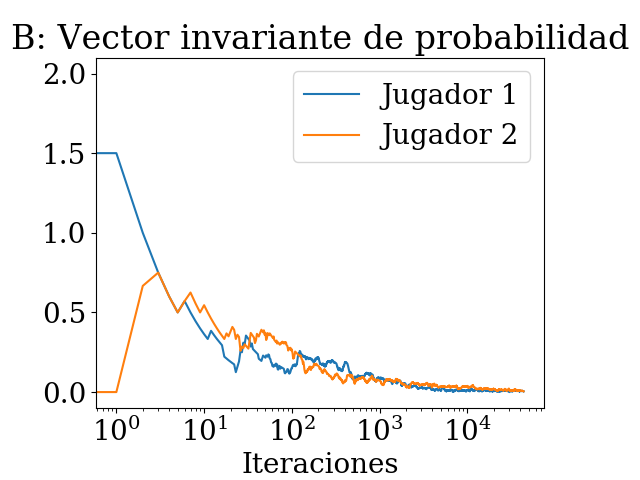
\includegraphics{../graphics/regret-matching/#1/procedimiento-B.png}
    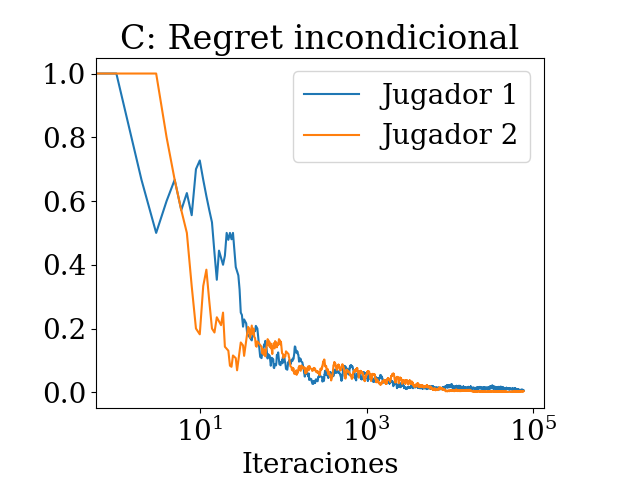
\includegraphics{../graphics/regret-matching/#1/procedimiento-C.png}
    }
\end{figure}
}

\begin{frame}{\Large Piedra, Papel o Tijera}
\Alert{Valor del juego ($u$):} $0$.
\vspace{.3cm}
\begin{center} \resizebox{.9\textwidth}{!}{
\begin{tabular}{l r r r}
    \toprule
    & \multicolumn{1}{c}{A} & \multicolumn{1}{c}{B} & \multicolumn{1}{c}{C} \\ \midrule
    Ganancia esperada $u(\sigma)$ & $-0,000012$ & $0,000004$ & $0,000022$ \\
    Explotabilidad $\varepsilon_{\sigma}$ &  $0,006$ & $0,010$ & $0,009$ \\
    Tiempo $T$ & $12,198$ & $0,345$ & $0,049$ \\
    Iteraciones $I$ & $4.519.054,1$ & $6.601,3$ &  $19.321,1$ \\
    $T/I$ & $2,70{\times}10^{-6}$ & $5,23{\times}10^{-5}$ & $2,54{\times}10^{-6}$ \\
    \bottomrule
\end{tabular}
} \end{center}
\graphicsRM{RPS}
\end{frame}

\begin{frame}{\Large Matching Pennies}
\begin{columns}
\column{.5\textwidth}
\begin{enumerate}
  \item Cada jugador posee una moneda y elige cara o sello.
  \item Misma elecci\'on: gana el primer jugador.
  \item Elecciones diferentes: gana el segundo jugador.
  \item Tabla de pagos.
\end{enumerate}
\begin{center}
\begin{tabular}{ c | c | c |}
 \multicolumn{1}{c}{} & \multicolumn{1}{c}{cara} & \multicolumn{1}{c}{sello}  \\ \cline{2-3}
 cara  &  1 & -1 \\ \cline{2-3}
 sello & -1 &  1 \\ \cline{2-3}
\end{tabular}
\end{center}

\column{.45\textwidth}
\begin{center}
\begin{tabular}{c}
{\cutpic{5mm}{.5\textwidth}{../images/cara.jpg}} \\
{\cutpic{5mm}{.5\textwidth}{../images/sello.jpg}}
\end{tabular}
\end{center}
\end{columns}
\end{frame}

\begin{frame}{\Large Matching Pennies}
\Alert{Valor del juego ($u$):} $0$.
\vspace{.3cm}
\begin{center} \resizebox{.9\textwidth}{!}{
\begin{tabular}{l r r r}
    \toprule
    & \multicolumn{1}{c}{A} & \multicolumn{1}{c}{B} & \multicolumn{1}{c}{C} \\ \midrule
    Ganancia esperada $u(\sigma)$ & $0,000$ & $0,000$ & $0,000$ \\
    Explotabilidad $\varepsilon_{\sigma}$ & $0,006$ & $0,006$ & $0,008$ \\
    Tiempo $T$ & $10,276$ & $0,777$ & $0,042$ \\
    Iteraciones $I$ & $3.892.550,4$ & $25.616,6$ & $16.260,5$   \\
    $T/I$ & $2,64{\times}10^{-6}$ & $3,03{\times}10^{-5}$ & $2,58{\times}10^{-6}$ \\
    \bottomrule
\end{tabular}
} \end{center}
\graphicsRM{matching-pennies}
\end{frame}


\begin{frame}{\Large Ficha vs. Domin\'o}

\vspace{.35cm}
\begin{columns}
\column{.45\textwidth}
\textbf{Jugador 1}
\vspace{.1cm}
\begin{center}
\begin{tikzpicture}
  \draw (0, 0) -- (3, 0);
  \draw (0, 1) -- (3, 1);
  \draw (0, 2) -- (3, 2);
  \draw (0, 0) -- (0, 2);
  \draw (1, 0) -- (1, 2);
  \draw (2, 0) -- (2, 2);
  \draw (3, 0) -- (3, 2);
  \visible<2>{\fill[gray!80] (0.25, 1.25) rectangle (1.75, 1.75);}
  \visible<3>{\fill[gray!80] (2.25, 0.25) rectangle (2.75, 1.75);}
  \visible<4>{\fill[gray!80] (1.25, 0.25) rectangle (2.75, 0.75);}
  \visible<5->{\fill[gray!80] (1.25, 0.25) rectangle (1.75, 1.75);}
\end{tikzpicture}
\end{center}
\column{.45\textwidth}
\textbf{Jugador 2}
\vspace{.1cm}
\begin{center}
\begin{tikzpicture}
  \draw (0, 0) -- (3, 0);
  \draw (0, 1) -- (3, 1);
  \draw (0, 2) -- (3, 2);
  \draw (0, 0) -- (0, 2);
  \draw (1, 0) -- (1, 2);
  \draw (2, 0) -- (2, 2);
  \draw (3, 0) -- (3, 2);
  \visible<6>{\fill (0.5, 1.5) circle (0.25);}
  \visible<7>{\fill (1.5, 1.5) circle (0.25);}
  \visible<8->{\fill (2.5, 0.5) circle (0.25);}
\end{tikzpicture}
\end{center}
\end{columns}
\vspace{1cm}
\visible<9->{%
\Alert{Resultado}
\begin{columns}
\column{.5\textwidth}
\begin{enumerate}
  \visible<9->{\item La ficha y el domin\'o no se superponen: gana el jugador 1.}
  \visible<10->{\item La ficha y el domin\'o s\'i se superponen: gana el jugador 2.}
\end{enumerate}
}
\column{.45\textwidth}
\visible<9->{%
\begin{tikzpicture}
  \draw (0, 0) -- (3, 0);
  \draw (0, 1) -- (3, 1);
  \draw (0, 2) -- (3, 2);
  \draw (0, 0) -- (0, 2);
  \draw (1, 0) -- (1, 2);
  \draw (2, 0) -- (2, 2);
  \draw (3, 0) -- (3, 2);
  \visible<9>{\fill (2.5, 0.5) circle (0.25);}
  \visible<9>{\fill[gray!80] (1.25, 0.25) rectangle (1.75, 1.75);}
  \visible<10->{\fill[gray!80] (0.25, 1.25) rectangle (1.75, 1.75);}
  \visible<10->{\fill (0.5, 1.5) circle (0.25);}
\end{tikzpicture}}
\end{columns}
\vspace{.82cm}
\end{frame}

\begin{frame}{\Large Ficha vs. Domin\'o}
\Alert{Valor del juego ($u$):} $\frac{1}{3}$.
\vspace{.3cm}
\begin{center} \resizebox{.9\textwidth}{!}{
\begin{tabular}{l r r r}
    \toprule
    & \multicolumn{1}{c}{A} & \multicolumn{1}{c}{B} & \multicolumn{1}{c}{C} \\ \midrule
    Ganancia esperada $u(\sigma)$ & $0,333$ & $0,334$ & $0,334$  \\
    Explotabilidad $\varepsilon_{\sigma}$ & $0,010$ & $0,007$ & $0,004$ \\
    Tiempo $T$ & $319,179$ & $11,275$ & $0,237$  \\
    Iteraciones $I$ & $108.319.272,4$ & $75.250,2$ & $84.318,5$ \\
    $T/I$ & $2,95 {\times} 10^{-6}$ & $1,50 {\times} 10^{-4}$ & $2,81 {\times} 10^{-6}$ \\
    \bottomrule
\end{tabular}
} \end{center}
\graphicsRM{domino}
\end{frame}

\newcommand{\soldier}[3]{
\node[circle,fill=#3,minimum size=.8mm] at #2 (head#1) {};
\node[color=#3, rounded corners=2pt,minimum height=1cm,minimum width=3mm,fill,below = 1pt of head#1] (body#1) {};
\draw[line width=.75mm,round cap-round cap, #3] ([shift={(1.5pt,-1pt)}]body#1.north east) --++(-90:4mm);
\draw[line width=.75mm,round cap-round cap, #3] ([shift={(-1.5pt,-1pt)}]body#1.north west)--++(-90:4mm);
\draw[thick,white,-round cap] (body#1.south) --++(90:4mm);
}

\begin{frame}{\Large Coronel Blotto}
\begin{columns}
\column{.45\textwidth}
\begin{itemize}
  \item $S$ soldados por jugador.
  \item $N$ campos de batalla.
\end{itemize}
\column{.45\textwidth}
\begin{itemize}
  \visible<6->{\item $u_1 = 1-2 = -1$}
  \visible<6->{\item $u_2 = 2-1 = 1$.}
\end{itemize}
\end{columns}
\begin{center}
\resizebox{.75\textwidth}{!}{
\begin{tikzpicture}
\node at (-2,4) {\textcolor{blue}{Jugador 1}};
\node at (6,4) {\textcolor{red}{Jugador 2}};
\visible<1>{
\soldier{1x1}{(-3, 2.5)}{blue}
\soldier{1x2}{(-2, 2.5)}{blue}
\soldier{1x3}{(-1, 2.5)}{blue}
\soldier{1x4}{(-2.5, 1)}{blue}
\soldier{1x3}{(-1.5, 1)}{blue}
}
\visible<1-2>{%
\soldier{2x1}{(5, 2.5)}{red}
\soldier{2x2}{(6, 2.5)}{red}
\soldier{2x3}{(7, 2.5)}{red}
\soldier{2x4}{(5.5, 1)}{red}
\soldier{2x5}{(6.5, 1)}{red}
}
\draw[rounded corners] (0, 0) rectangle (4, 1.75);
\draw[fill=gray] (0, 0) rectangle (4, .25);
\draw[rounded corners] (0, 2.5) rectangle (4, 4.25);
\draw[fill=gray] (0, 2.5) rectangle (4, 2.75);
\draw[rounded corners] (0, -2.5) rectangle (4, -0.75);
\draw[fill=gray] (0, -2.5) rectangle (4, -2.25);
\visible<2-3>{%
\soldier{3x1}{(0.5, 3.85)}{blue}
\soldier{3x2}{(1.25, 3.85)}{blue}
}
\visible<2-4>{%
\soldier{3x3}{(0.5, 1.35)}{blue}
\soldier{3x4}{(1.25, 1.35)}{blue}
}
\visible<2-4>{%
\soldier{3x5}{(0.5, -1.15)}{blue}
}
\visible<3-4>{%
\soldier{4x1}{(3.5, 1.35)}{red}
\soldier{4x2}{(2.75, 1.35)}{red}
\soldier{4x3}{(2, 1.35)}{red}
}
\visible<3-4>{%
\soldier{4x4}{(3.5, -1.15)}{red}
\soldier{4x5}{(2.75, -1.15)}{red}
}
\visible<4->{%
\soldier{w1}{(1.625, 3.85)}{blue}
\soldier{w2}{(2.375, 3.85)}{blue}
}
\visible<5->{%
\soldier{w3}{(1.25, 1.35)}{red}
\soldier{4x2}{(2.75, 1.35)}{red}
\soldier{4x3}{(2, 1.35)}{red}
}
\visible<5->{%
\soldier{4x4}{(1.625, -1.15)}{red}
\soldier{4x5}{(2.375, -1.15)}{red}
}
\end{tikzpicture}
}
\end{center}
\end{frame}

\begin{frame}{\Large Coronel Blotto}
\Alert{Valor del juego ($u$):} $0$.
\vspace{.3cm}
\begin{center} \resizebox{.9\textwidth}{!}{
\begin{tabular}{l r r r}
    \toprule
    & \multicolumn{1}{c}{A} & \multicolumn{1}{c}{B} & \multicolumn{1}{c}{C} \\ \midrule
    Ganancia esperada $u(\sigma)$ & $0,000219$ & $0,000150$ & $0,000024$ \\
    Explotabilidad $\varepsilon_{\sigma}$ & $0,010$ & $0,010$ & $0,009$  \\
    Tiempo $T$ &  $875,533$ &  $70,453$ & $0,166$ \\
    Iteraciones $I$ &  $190.222.305,3$ & $58.794,4$  & $48.613,5$ \\
    $T/I$ & $4,60{\times}10^{-6}$ & $1,20{\times}10^{-3}$ & $3,41{\times}10^{-6}$ \\
    \bottomrule
\end{tabular}
} \end{center}
\graphicsRM{blotto-game}
\end{frame}

\tikzset{onslide/.code args={<#1>#2}{%
  \only<#1>{\pgfkeysalso{#2}}
}}

\begin{frame}{\Large Forma Normal y Regret Matching: Conclusiones}
\begin{enumerate}
  \item El equilibrio de Nash es un concepto de soluci\'on satisfactorio en juegos en forma normal de dos jugadores de suma cero.
  \item Los algoritmos de Regret Matching permiten encontrar aproximaciones de un equilibrio de Nash en este tipo de juegos.
  \item El procedimiento ``regret condicional'' necesita mayor n\'umero de iteraciones, y por lo tanto mayor tiempo, para converger.
  \item El procedimiento ``vector invariante de probabilidad'' es el procedimiento con las iteraciones m\'as costosas.
  \item El procedimiento ``regret incondicional'' es el m\'as eficiente.
\end{enumerate}
\end{frame}

\begin{frame}
  \centering{\resizebox{!}{.5cm}{\Alert{Forma Extensiva}}}
\end{frame}

\begin{frame}{\Large Forma Extensiva: Modelo}
\begin{columns}
\column{.5\textwidth}
\Alert{Juegos secuenciales}
\vspace{.2cm}

\visible<2->{%
\resizebox{\textwidth}{!}{
\begin{tikzpicture}[
player1/.style={circle, fill=blue, thick, minimum size = 4mm},
player2/.style={circle, fill=red, thick, minimum size=4mm},
chance/.style={circle, fill=gray, thick, minimum size=4mm},
terminal/.style={rectangle, draw=black, fill=black, thick, minimum size=2mm},
level 1/.style={sibling distance=25mm, level distance=20mm},
level 2/.style={sibling distance=25mm, level distance=20mm},
level 3/.style={sibling distance=12.5mm, level distance=15mm},
level 4/.style={level distance=30mm}
]
\visible<2->{
\node[player1] (root) {}
  child { node (L) [player2]  {}
      child { [onslide=<2>{color=white}] node (A) [player1, onslide=<2>{color=white}]  {}
            child {[onslide=<2-3>{color=white}] node [terminal, onslide=<2-3>{color=white}] [label=below:{$(0,0)$}] {}
                edge from parent node[left] {$a$} }
            child {[onslide=<2-3>{color=white}] node [terminal, onslide=<2-3>{color=white}] [label=below:{$(2,4)$}] {}
                edge from parent node[right] {$b$}}
            edge from parent node[left] {A\, \, }
      }
      child { [onslide=<2>{color=white}] node (B) [player1, onslide=<2>{color=white}] {}
          child {[onslide=<2-3>{color=white}] node (t1) [terminal, onslide=<2-3>{color=white}] [label=below:{$(2,4)$}] {}
              edge from parent node[left] {$a$} }
          child {[onslide=<2-3>{color=white}] node (t2) [terminal, onslide=<2-3>{color=white}] [label=below:{$(0,0)$}] {}
              edge from parent node[right] {$b$} }
          edge from parent node[right] {B}
      }
      child { [onslide=<2>{color=white}] node (C) [chance, onslide=<2>{color=white}] {}
          child {[onslide=<2-4>{color=white}] node (t3) [terminal, onslide=<2-4>{color=white}] [label=below:{$(4,4)$}] {}
              edge from parent node[left] {$\visible<15>{\frac{1}{2}}\ c$} }
          child {[onslide=<2-4>{color=white}] node (t4) [terminal, onslide=<2-4>{color=white}] [label=below:{$(0,0)$}] {}
              edge from parent node[right] {$s\ \visible<15>{\frac{1}{2}}$} }
          edge from parent node[right] {\, \, C}
      }
      edge from parent node[left] [label=left:{L}] {}
  }
  child { node (R) [terminal] [label=below:{$(1,1)$}] {}
      edge from parent node[right] [label=right:{R}] {}
  }
;}
\visible<3->{\draw[dotted] (A) -- (B);}

\visible<8>{\draw[thick] (C) ellipse (.6cm and .6 cm);}
\visible<10>{\draw[thick, blue] ($(A)!0.5!(B)$) ellipse (2cm and .65cm);}
\visible<10>{\draw[thick, blue] (root) ellipse (.6cm and .6 cm);}
\visible<11>{\draw[thick, red] (L) ellipse (.6cm and .6 cm);}

\node (c1) at ($(t1)!0.5!(t2)$) {};
\node (c2) [below of=c1] {};
\node (c0) at ($(c1)!0.3!(c2)$) {};
\visible<13>{\draw[dashed] (c0) ellipse (4cm and .75cm);}
\node (R1) [below of=R] {};
\node (R0) at ($(R)!0.3!(R1)$) {};
\visible<13>{\draw[dashed] (R0) ellipse (.75cm and .6cm);}
\visible<15>{\draw[dashed] ($(t3)!0.5!(t4)!0.25!(C)$) ellipse (1.5cm and 1.5cm);}
\end{tikzpicture}
}}

\vspace{.1cm}
\visible<16->{\Alert{Perfect Recall}\\
Se recuerda de forma perfecta todo lo que se ha visto.}

\column{.45\textwidth}
\visible<6->{\Alert{Elementos}}

\begin{enumerate}
  \visible<6->{\onslide<6>{\item Historias o nodos.\\Ej: $\emptyset$, $LA, LBb, R$.}}
  \visible<7->{\onslide<7-8>{\item Funci\'on que asigna a cada historia (nodo) no terminal un jugador.}}
  \visible<8->{
    \begin{itemize}
      \onslide<8>{\item Nodos de azar.}
    \end{itemize}
  }
  \visible<9->{\onslide<9-11>{\item Conjuntos de informaci\'on.}}
  \visible<12->{\onslide<12-13>{\item Funci\'on que asigna por cada historia (nodo) terminal y cada jugador una utilidad.}}
  \visible<14->{\onslide<14-15>{\item Distribuci\'on de probabilidad sobre el conjunto de acciones en cada nodo de azar.}}
\end{enumerate}
\end{columns}
\end{frame}

\begin{frame}{\Large Forma Extensiva: Estrategias}
\begin{columns}
\column{.45\textwidth}
\resizebox{\textwidth}{!}{
\begin{tikzpicture}[
player1/.style={circle, fill=blue, thick, minimum size = 4mm},
player2/.style={circle, fill=red, thick, minimum size=4mm},
chance/.style={circle, fill=gray, thick, minimum size=4mm},
terminal/.style={rectangle, draw=black, fill=black, thick, minimum size=2mm},
level 1/.style={sibling distance=25mm, level distance=20mm},
level 2/.style={sibling distance=25mm, level distance=20mm},
level 3/.style={sibling distance=12.5mm, level distance=15mm},
level 4/.style={level distance=30mm}
]
\node[player1] (root) {}
  child {node (L) [player2]  {}
      child {node (A) [player1]  {}
            child {node [terminal] [label=below:{$(0,0)$}] {}
                edge from parent node[left] {$a$} }
            child {node [terminal] [label=below:{$(2,4)$}] {}
                edge from parent node[right] {$b$}}
            edge from parent node[left] {A\, \, }
      }
      child {node (B) [player1] {}
          child {node (t1) [terminal] [label=below:{$(2,4)$}] {}
              edge from parent node[left] {$a$} }
          child {node (t2) [terminal] [label=below:{$(0,0)$}] {}
              edge from parent node[right] {$b$} }
          edge from parent node[right] {B}
      }
      child {node (C) [chance] {}
          child {node (t3) [terminal] [label=below:{$(4,4)$}] {}
              edge from parent node[left] {$c$} }
          child {node (t4) [terminal] [label=below:{$(0,0)$}] {}
              edge from parent node[right] {$s$} }
          edge from parent node[right] {\, \, C}
      }
      edge from parent node[left] [label=left:{L}] {}
  }
  child {node (R) [terminal] [label=below:{$(1,1)$}] {}
      edge from parent node[right] [label=right:{R}] {}
  }
;
\draw[dotted] (A) -- (B);
\end{tikzpicture}
}

\vspace{.2cm}
\Alert{Forma Normal}

\vspace{.1cm}
\begin{tabular}{c|c|c|c|}
\multicolumn{1}{c}{} & \multicolumn{1}{c}{A} & \multicolumn{1}{c}{B\raisebox{1pt}{\mymark{pB}}} & \multicolumn{1}{c}{C} \\ \cline{2-4}
(L, $a$) & $0, 0$ & $2, 4$ & $2, 2$ \\ \cline{2-4}
(L,\raisebox{-5pt}{\tikzmark{pA}} $b$) &  $2, 4$ & $0, 0$ & $2, 2$ \\ \cline{2-4}
(R, $a$) & $1, 1$ & $1, 1$ & $1, 1$ \\ \cline{2-4}
(R, $b$) & $1, 1$ & $1, 1$ & $1, 1$ \\ \cline{2-4}
\end{tabular}
\ellipse{3}{13pt}{25pt}{pA}
\ellipse{4}{30pt}{6pt}{pB}

\column{.5\textwidth}
\visible<2->{\Alert{Estrategias}}
\begin{enumerate}
  \visible<2->{\item Estrategias Puras.}
  \visible<5->{\item Estrategias Mixtas.}
  \visible<6->{\begin{tabular}{@{}cccc@{}}
  \cmidrule{1-4}
  (L, $a$) & (L, $b$) & (R, $a$) & (R, $b$) \\
  $0.45$ & $0.30$ & $0.00$ &  $0.25$ \\ \cmidrule{1-4}
  \end{tabular}}
  \visible<6->{\begin{tabular}{@{}ccc@{}}
  \cmidrule{1-3}
  A & B & C \\
  $0.25$ & $0.25$ & $0.50$ \\
  \cmidrule{1-3}
  \end{tabular}}
  \visible<7->{\item Estrategias de Comportamiento.}
  \visible<8->{\begin{tabular}{@{}cccc@{}}
  \cmidrule(r){1-2} \cmidrule(l){3-4}
  L  & R & $a$ & $b$ \\
  $0.65$ & $0.35$ & $0.40$ &  $0.60$ \\ \cmidrule(r){1-2} \cmidrule(l){3-4}
  \end{tabular}}
\end{enumerate}
\vspace{.2cm}
\visible<9->{\Alert{Equilibrio de Nash} \\
Mejor respuesta frente a la estrategias de sus oponentes.}

\end{columns}
\end{frame}

% \begin{frame}{\Large Forma Extensiva}
% \begin{columns}
% \column{.4\textwidth}
% \visible<2->{\Alert{Perfect Recall}}
% \vspace{.3cm}
% \begin{enumerate}
%   \visible<3->{\item El jugador recuerda lo que sab\'ia.}
%   \visible<4->{\item El jugador recuerda lo que eligi\'o.}
% \end{enumerate}
% \vspace{.5cm}
% \visible<11->{En un juego con perfect recall las estrategias mixtas y de comportamiento tienen el mismo poder expresivo.}
% \visible<5->{%
% \column{.575\textwidth}
% \resizebox{\textwidth}{!}{\begin{tikzpicture}[
% chance/.style={circle, fill=gray, thick, minimum size = 4mm},
% player1/.style={circle, fill=blue, thick, minimum size = 4mm},
% player2/.style={circle, fill=red, thick, minimum size=4mm},
% terminal/.style={rectangle, draw=black, fill=black, thick, minimum size=2mm},
% level 1/.style={sibling distance=50mm, level distance=25mm},
% level 2/.style={sibling distance=25mm, level distance=25mm},
% level 3/.style={sibling distance=20mm, level distance=20mm},
% ]

% \node[chance] [label = {Nodo de azar}] {}
%   child { [onslide=<5>{color=white}] node[player1, onslide=<5>{color=white}] [label=above:{A}] {}
%     child { [onslide=<5-6>{color=white}] node[terminal, onslide=<5-6>{color=white}] [label=below:{$1$}] {}
%       edge from parent node[left] {P}
%     }
%     child { [onslide=<5-6>{color=white}] node (A) [player1, onslide=<5-6>{color=white}] [label=above:{B}] {}
%       child { [onslide=<5-9>{color=white}] node[terminal, onslide=<5-9>{color=white}] [label=below:{$2$}] {}
%         edge from parent node[left] {M}
%       }
%       child { [onslide=<5-9>{color=white}] node[terminal, onslide=<5-9>{color=white}] [label=below:{$0$}] {}
%         edge from parent node[right] {I}
%       }
%       edge from parent node[right] {C}
%     }
%     edge from parent node[left] [label=above:{$2, 1\ \ $}] {}
%   }
%   child { [onslide=<5>{color=white}] node[player2, onslide=<5>{color=white}] [label=above:{Z}] {}
%     child { [onslide=<5-7>{color=white}] node (C) [terminal, onslide=<5-7>{color=white}] [label=below:{$-1$}] {}
%       edge from parent node[left] {P}
%     }
%     child { [onslide=<5-7>{color=white}] node (B) [player1, onslide=<5-7>{color=white}] [label=above:{B}] {}
%       child { [onslide=<5-9>{color=white}] node[terminal, onslide=<5-9>{color=white}] [label=below:{$-2$}] {}
%         edge from parent node[left] {M}
%       }
%       child { [onslide=<5-9>{color=white}] node[terminal, onslide=<5-9>{color=white}] [label=below:{$0$}] {}
%         edge from parent node[right] {I}
%       }
%       edge from parent node[right] {C}
%     }
%     edge from parent node[right] [label=above:{$\ \ 1, 2$}] {}
%   }
% ;

% \visible<9->{\draw[dashed] (A.east) .. controls ++(135:-18mm) and ++(45:-18mm) .. (B.west);}
% \end{tikzpicture}}}
% \end{columns}
% \end{frame}

\begin{frame}{\Large Kuhn Poker}
\resizebox{\textwidth}{!}{
\begin{tikzpicture}[
chance/.style={circle, draw=black, fill=gray, thick, minimum size = 6mm},
player1/.style={circle, draw=black, solid, thick, minimum size = 4mm},
player2/.style={circle, thick, minimum size=4mm},
terminal/.style={rectangle, draw=black, solid, fill=black, thick, minimum size=2mm},
level 1/.style={sibling distance=26mm, level distance=25mm},
level 2/.style={sibling distance=13mm, level distance=14mm},
level 3/.style={sibling distance=6.5mm, level distance=14mm},
]
\node[chance] [label=above:{Nodo de azar}] {} {
  child {node [player1] (P1) [label=above:{$1, 2$}]{}
    child { node [player2] [draw=red, fill=red] {}
        child { node [terminal] [label=below:{$-1$}] {}
            edge from parent [dashed] {} }
        child { node [player1] (A) {}
            child { node [terminal] [label=below:{$-1$}] {}
                edge from parent [dashed] {} }
            child { node [terminal] [label=below:{$-2$}] {}
                edge from parent [solid, double] {} }
            edge from parent [solid, double] {}
        }
        edge from parent [dashed] {}
    }
    child { node [player2] [draw=red] {}
        child { node [terminal] [label=below:{$1$}] {}
            edge from parent [dashed] {} }
        child { node [terminal] [label=below:{$-2$}] {}
            edge from parent [solid, double] {} }
        edge from parent [solid, double] {}
    }
  }
  child {node [player1] (P2) [label=above:{$\ \ 1, 3$}]{}
    child { node [player2] [draw=blue, fill=blue] {}
        child { node [terminal] [label=below:{$-1$}] {}
            edge from parent [dashed] {} }
        child { node [player1] (B) {}
            child { node [terminal] [label=below:{$-1$}] {}
                edge from parent [dashed] {} }
            child { node [terminal] [label=below:{$-2$}] {}
                edge from parent [solid, double] {} }
            edge from parent [solid, double] {}
        }
        edge from parent [dashed] {}
    }
    child { node [player2] [draw=blue] {}
        child { node [terminal] [label=below:{$1$}] {}
            edge from parent [dashed] {} }
        child { node [terminal] [label=below:{$-2$}] {}
            edge from parent [solid, double] {} }
        edge from parent [solid, double] {}
    }
  }
  child {node [player1] (P3) [label=135:{$2, 1$}]{}
    child { node [player2] [draw=green, fill=green] {}
        child { node [terminal] [label=below:{$1$}] {}
            edge from parent [dashed] {} }
        child { node [player1] (C) {}
            child { node [terminal] [label=below:{$-1$}] {}
                edge from parent [dashed] {} }
            child { node [terminal] [label=below:{$2$}] {}
                edge from parent [solid, double] {} }
            edge from parent [solid, double] {}
        }
        edge from parent [dashed] {}
    }
    child { node [player2] [draw=green] {}
        child { node [terminal] [label=below:{$1$}] {}
            edge from parent [dashed] {} }
        child { node [terminal] [label=below:{$2$}] {}
            edge from parent [solid, double] {} }
        edge from parent [solid, double] {}
    }
  }
  child {node [player1] (P4) [label=45:{$2, 3$}]{}
    child { node [player2] [draw=blue, fill=blue]{}
        child { node [terminal] [label=below:{$-1$}] {}
            edge from parent [dashed] {} }
        child { node [player1] (D) {}
            child { node [terminal] [label=below:{$-1$}] {}
                edge from parent  [dashed] {} }
            child { node [terminal] [label=below:{$-2$}] {}
                edge from parent [solid, double] {} }
            edge from parent [solid, double] {}
        }
        edge from parent [dashed] {}
    }
    child { node [player2] [draw=blue] {}
        child { node [terminal] [label=below:{$1$}] {}
            edge from parent [dashed] {} }
        child { node [terminal] [label=below:{$-2$}] {}
            edge from parent [solid, double] {} }
        edge from parent [solid, double] {}
    }
  }
  child {node [player1] (P5) [label=above:{$3, 1\ \ $}]{}
    child { node [player2] [draw=green, fill=green] {}
        child { node [terminal] [label=below:{$1$}] {}
            edge from parent [dashed] {} }
        child { node [player1] (E) {}
            child { node [terminal] [label=below:{$-1$}] {}
                edge from parent [dashed] {} }
            child { node [terminal] [label=below:{$2$}] {}
                edge from parent [solid, double] {} }
            edge from parent [solid, double] {}
        }
        edge from parent [dashed] {}
    }
    child { node [player2] [draw=green] {}
        child { node [terminal] [label=below:{$1$}] {}
            edge from parent [dashed] {} }
        child { node [terminal] [label=below:{$2$}] {}
            edge from parent [solid, double] {} }
        edge from parent [solid, double] {}
    }
  }
  child {node [player1] (P6) [label=above:{$3, 2$}]{}
    child { node [player2]  [draw=red, fill=red] {}
        child { node [terminal] [label=below:{$1$}] {}
            edge from parent [dashed] {} }
        child { node [player1] (F) {}
            child { node [terminal] [label=below:{$-1$}] {}
                edge from parent [dashed] {}}
            child { node [terminal] [label=below:{$2$}] {}
                edge from parent [solid, double] {} }
            edge from parent [solid, double] {}
        }
        edge from parent [dashed] {}
    }
    child { node [player2]  [draw=red] {}
        child { node [terminal] [label=below:{$1$}] {}
            edge from parent [dashed] {} }
        child { node [terminal] [label=below:{$2$}] {}
            edge from parent [solid, double] {} }
        edge from parent [solid, double] {}
    }
  }
};
\draw[dotted]
(A.south) .. controls ++(-45:10mm) and ++(45:-10mm) .. (B.south);
\draw[dotted]
(C.south) .. controls ++(-45:10mm) and ++(45:-10mm) .. (D.south);
\draw[dotted]
(E.south) .. controls ++(-45:10mm) and ++(45:-10mm) .. (F.south);
\draw[dotted] (P1.east) -- (P2.west);
\draw[dotted] (P3.east) -- (P4.west);
\draw[dotted] (P5.east) -- (P6.west);
\end{tikzpicture}}
% \visible<3->{\Alert{Interrogantes}}
% \begin{enumerate}[--]
%   \visible<4->{\item ?`Qu\'e es una estrategia?}
%   \visible<5->{\item ?`Es posible ``enga\~nar'' al oponente?}
% \end{enumerate}
\end{frame}

\begin{frame}{Counterfactual Regret Minimization (CFR)}
\begin{enumerate}
\item El \'arbol del juego se recorre repetidamente. %La m\'aquina juega contra s\'i misma a lo largo del tiempo.}}
\item Inicia con una estrategia uniforme en cada conjunto de informaci\'on.
\item En cada iteraci\'on se elige una mejor estrategia revisando las decisiones pasadas, utilizando las m\'etricas de regret.
\item La estrategia promedio converge a un equilibrio de Nash; en la pr\'actica el algoritmo es detenido despu\'es de cierto n\'umero de iteraciones.
\end{enumerate}
\visible<2->{\Alert{?`C\'omo se mejora la estrategia en cada iteraci\'on?}}
\begin{enumerate}[--]
\visible<2->{\item Sumar el regret contrafactual que se tiene en cada conjunto de informaci\'on por cada acci\'on.}
\visible<2->{\item \textbf{Regret contrafactual}: cu\'anto mejor lo habr\'ia hecho en todos los juegos hasta ahora si siempre hubiera jugado esta acci\'on en este conjunto de informaci\'on.}
\visible<2->{\item \textbf{Regret Matching}: en la nueva estrategia las acciones son elegidas con probabilidades proporcionales a los regrets positivos.}
\end{enumerate}
\end{frame}

\begin{frame}{\Large CFR: Experimentos}
\begin{enumerate}
  \item CFR con muestreo en los nodos de azar.
  \item Implementaci\'on propia del algoritmo.
  \begin{itemize}
    \item Input: definici\'on del juego.
    \item \textbf{Definici\'on del juego}: implementaci\'on de las funciones que permiten recorrer el \'arbol de forma \'implicita.
  \end{itemize}
  \item Tres clases de juegos, cada uno con diferentes par\'ametros.
  \item 10 horas de entrenamiento.
  \item Gr\'afica del regret con respecto al n\'umero de iteraciones.
  \item Verificaci\'on: la explotabilidad mide la distancia entre la estrategia actual y un equilibrio de Nash.
  \item Un juego se considera resuelto si la explotabilidad es menor que el $1\%$ de la m\'inima ganancia positiva posible.
    % \begin{columns}%
    % \column{.45\textwidth}%
    % \begin{itemize}
    %   \setlength{\itemsep}{0pt}
    %   \visible<8->{\item Instancia estudiada.}
    %   \visible<9->{\item N\'umero de nodos del \'arbol.}
    %   \visible<10->{\item N\'umero de conjuntos de informaci\'on.}
    %   \visible<11->{\item N\'umero de iteraciones.}
    % \end{itemize}%
    % \column{.45\textwidth}%
    % \begin{itemize}
    %   \setlength{\itemsep}{0pt}
    %   \visible<12->{\item Ganancia esperada del primer jugador de la estrategia calculada.}
    %   \visible<13->{\item Explotabilidad.}
    %   \visible<14->{\item Se resolvi\'o o no la instancia.}
    % \end{itemize}
    % \end{columns}
\end{enumerate}
\end{frame}

\definecolor{ao}{rgb}{0.0, 0.5, 0.0}
\newcommand{\cmark}{\textcolor{ao}{\ding{51}}}
\newcommand{\xmark}{\textcolor{red}{\ding{55}}}

\begin{frame}{\Large One Card Poker (OCP)}
\begin{enumerate}[--]
  \item Generalizaci\'on del Juego Kuhn Poker.
  \item $N$: n\'umero de cartas.
  \item OCP$(N)$.
\end{enumerate}
\vspace{.3cm}

\visible<2->{%
\Alert{Tabla de Resultados}
\begin{center}
\resizebox{.95\textwidth}{!}{\begin{tabular}{lrrrrrc}
    \toprule
    Juego & $N$ & $I$ & Iteraciones & $u(\sigma)$ & $\varepsilon_{\sigma}$ (\%) & Resuelto\\ \midrule
    OCP$(3)$        &          55 &      12 & 1.181.763.638 & -0,056 & 0,0098 & \cmark \\
    OCP$(12)$       &       1.189 &      48 & 1.147.919.240 & -0,062 & 0,0032 & \cmark \\
    OCP$(50)$       &      22.051 &     200 & 1.145.291.974 & -0,058 & 0,0099 & \cmark \\
    OCP$(200)$      &     358.201 &     800 & 1.128.993.847 & -0,056 & 0,0078 & \cmark \\
    OCP$(1000)$     &   8.991.001 &   4.000 & 1.087.573.694 & -0,056 & 0,0098 & \cmark \\
    OCP$(5000)$     & 224.955.001 &  20.000 & 1.038.367.354 & -0,056 & 0,0241 & \cmark \\
    \bottomrule
\end{tabular}}
\end{center}}
\end{frame}

\begin{frame}{\Large One Card Poker (OCP)}
\begin{center}
\resizebox{.9\textwidth}{!}{\begin{tabular}{@{}ccc@{}}
  {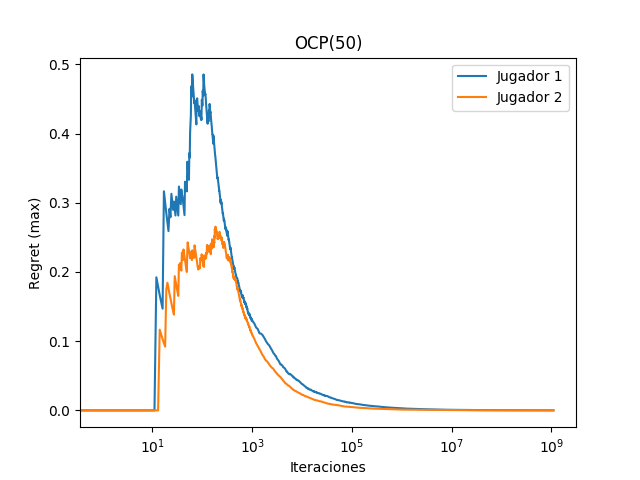
\includegraphics{../graphics/cfr/ocp/OCP(50).png}} &
  {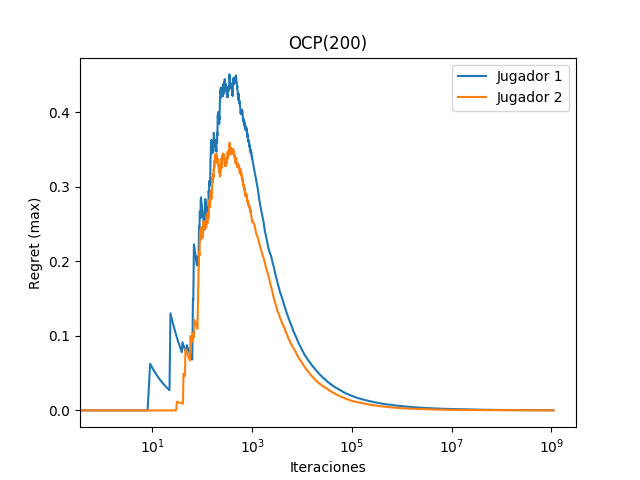
\includegraphics{../graphics/cfr/ocp/OCP(200).png}}
\end{tabular}}

\resizebox{.9\textwidth}{!}{\begin{tabular}{@{}ccc@{}}
  {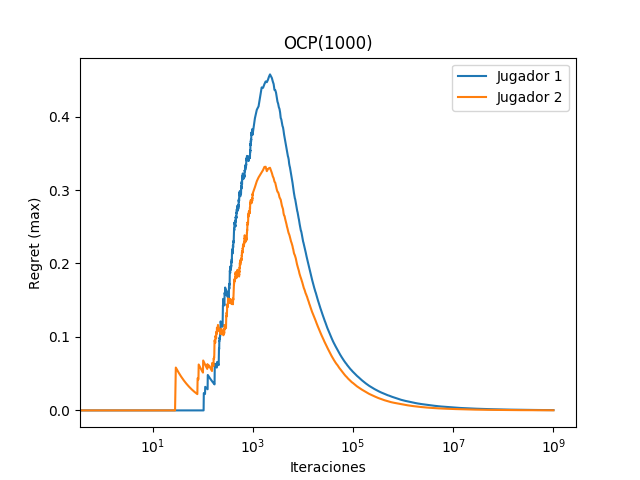
\includegraphics{../graphics/cfr/ocp/OCP(1000).png}} &
  {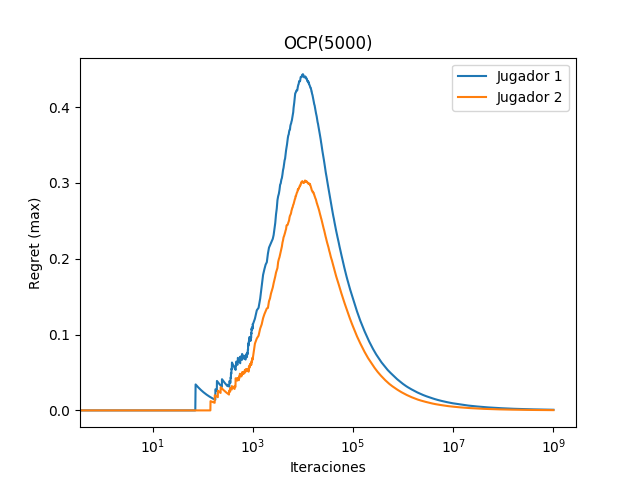
\includegraphics{../graphics/cfr/ocp/OCP(5000).png}}
\end{tabular}}
\end{center}
\end{frame}

\begin{frame}{\Large Dudo}
\begin{enumerate}[--]
  \item Juego de dados y apuestas.
  \item $K$: n\'umero de caras de los dados.
  \item $D_1, D_2$: n\'umero de dados del primer y segundo jugador, respectivamente.
  \item Dudo$(K, D_1, D_2)$.
\end{enumerate}

\visible<2-3>{%
\Alert{Tabla de Resultados}
\begin{center}
\resizebox{.95\textwidth}{!}{\begin{tabular}{lrrrrrc}
    \toprule
    Juego & $N$ & $I$ & Iteraciones & $u(\sigma)$ & $\varepsilon_{\sigma}$ (\%) & Resuelto \\ \midrule
    \onslide<2>{Dudo$(4, 1, 1)$ &         8.177 &         512 & 18.697.532 & -0,125 &  0,0259 & \cmark} \\
    \onslide<2>{Dudo$(4, 1, 2)$ &       327.641 &      14.366 &  1.215.600 & -0,508 &  0,0971 & \cmark} \\
    \onslide<2>{Dudo$(4, 2, 1)$ &       327.641 &      14.366 &  1.213.799 &  0,552 &  0,3701 & \cmark} \\
    Dudo$(4, 2, 2)$ &    13.107.101 &      327.680 &     63.109 & 0,0069 &  2,1132 & \xmark \\
    \onslide<2>{Dudo$(5, 1, 1)$ &        51.176 &       2.560 &  4.521.208 & -0,120 &  0,1186 & \cmark} \\
    \onslide<2>{Dudo$(5, 1, 2)$ &     4.915.126 &     163.840 &    151.235 & -0,565 &  0,6197 & \cmark} \\
    \onslide<2>{Dudo$(5, 2, 1)$ &     4.915.126 &     163.840 &    143.698 &  0,581 &  0,0122 & \cmark} \\
    Dudo$(5, 2, 2)$ &   471.858.976 &   7.864.320 &      3.826 &  0,836 & 15,1963 & \xmark \\
    \onslide<2>{Dudo$(6, 1, 1)$ &       294.877 &      12.288 &  1.067.782 & -0,111 &  0,0975 & \cmark} \\
    Dudo$(6, 1, 2)$ &    66.060.163 &   1.769.472 &     17.702 & -0,593 &  4,5781 & \xmark \\
    Dudo$(6, 2, 1)$ &    66.060.163 &   1.769.472 &     17.221 &  0,592 &  3,9594 & \xmark \\
    \bottomrule
\end{tabular}}
\end{center}}
\end{frame}

\begin{frame}{\Large Dudo}
\begin{center}
\resizebox{.9\textwidth}{!}{\begin{tabular}{@{}ccc@{}}
  {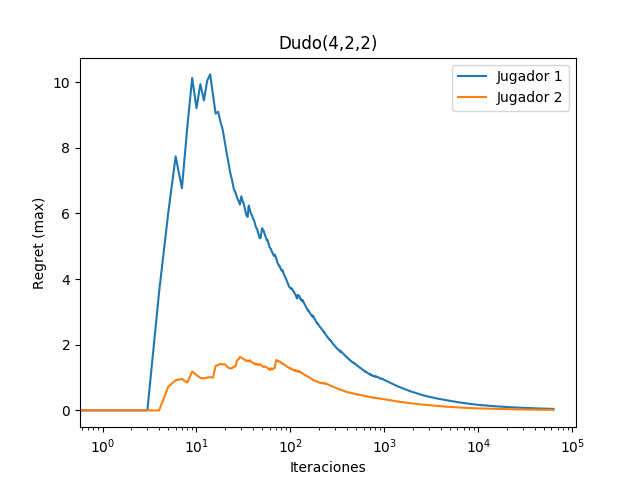
\includegraphics{../graphics/cfr/dudo/Dudo(4,2,2).png}} &
  {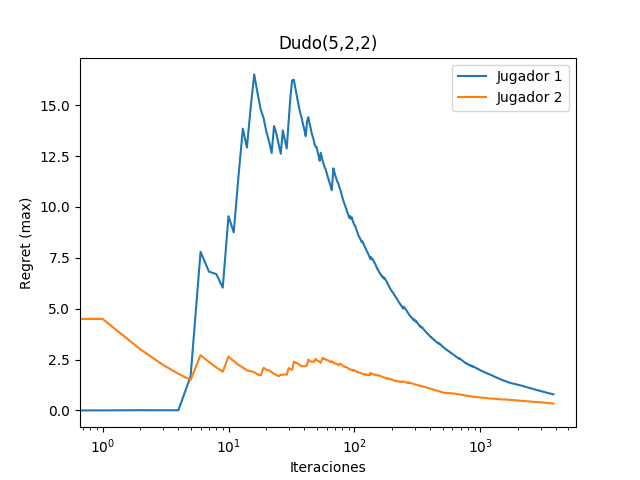
\includegraphics{../graphics/cfr/dudo/Dudo(5,2,2).png}}
\end{tabular}}

\resizebox{.9\textwidth}{!}{\begin{tabular}{@{}ccc@{}}
  {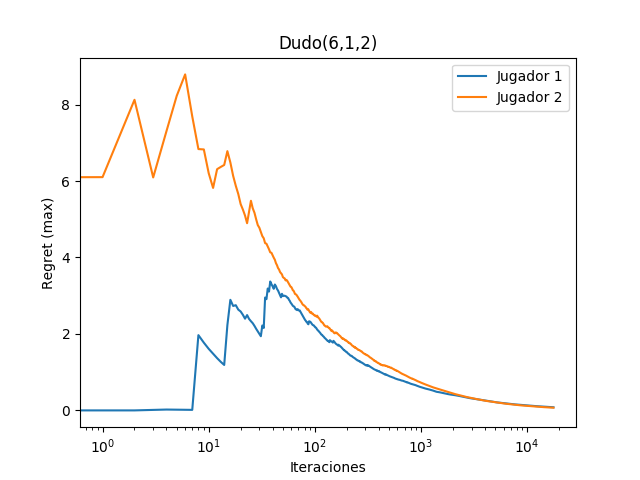
\includegraphics{../graphics/cfr/dudo/Dudo(6,1,2).png}} &
  {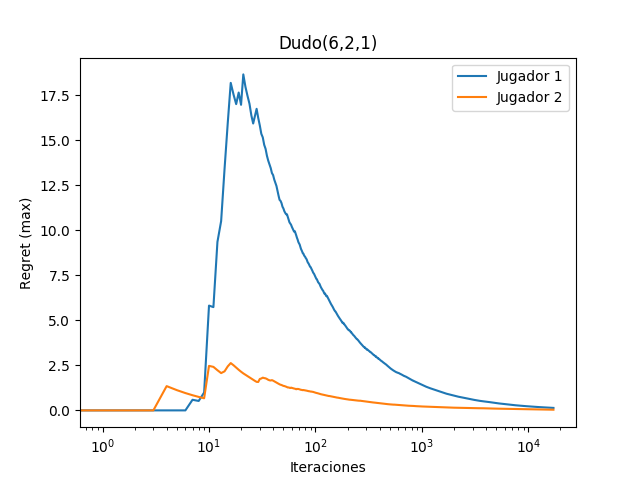
\includegraphics{../graphics/cfr/dudo/Dudo(6,2,1).png}}
\end{tabular}}
\end{center}
\end{frame}

\begin{frame}{\Large Domin\'o}
\begin{enumerate}[--]
  \item Versi\'on para dos jugadores.
  \item $M$: m\'aximo n\'umero de puntos en una cara de una pieza.
  \item $N$: n\'umero de piezas de la mano inicial para cada jugador.
  \item Domino$(M, N)$.
\end{enumerate}
\vspace{.3cm}

\visible<2-3>{%
\Alert{Tabla de Resultados}
\begin{center}
\resizebox{.95\textwidth}{!}{\begin{tabular}{lrrrrrc}
    \toprule
    Juego & $N$ & $I$ & Iteraciones & $u(\sigma)$ & $\varepsilon_{\sigma}$ (\%) & Resuelto \\ \midrule
    \onslide<2>{Domino$(2, 2)$ &         7.321 &     102 & 540.186.366 & 2,4000 & 0,0000 & \cmark} \\
    \onslide<2>{Domino$(3, 2)$ &    46.534.657 &  88.947 & 400.047.334 & 2,8767 & 0,0315 & \cmark} \\
    \onslide<2>{Domino$(3, 3)$ &   246.760.993 & 107.854 &  72.492.951 & 2,1539 & 0,3854 & \cmark} \\
    Domino$(3, 4)$ & 1.547.645.185 & 104.050 &  11.213.463 & 3,2034 & 1,4871 & \xmark \\
    \bottomrule
\end{tabular}}
\end{center}}
\end{frame}

\begin{frame}{\Large Domin\'o}
\begin{center}
\resizebox{.9\textwidth}{!}{\begin{tabular}{@{}ccc@{}}
  {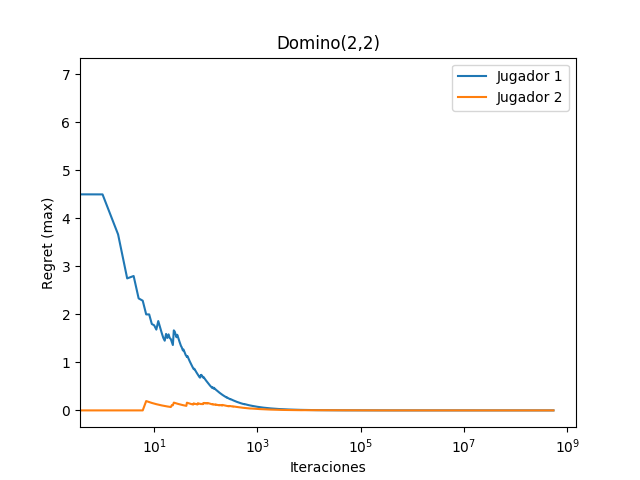
\includegraphics{../graphics/cfr/domino/Domino(2,2).png}} &
  {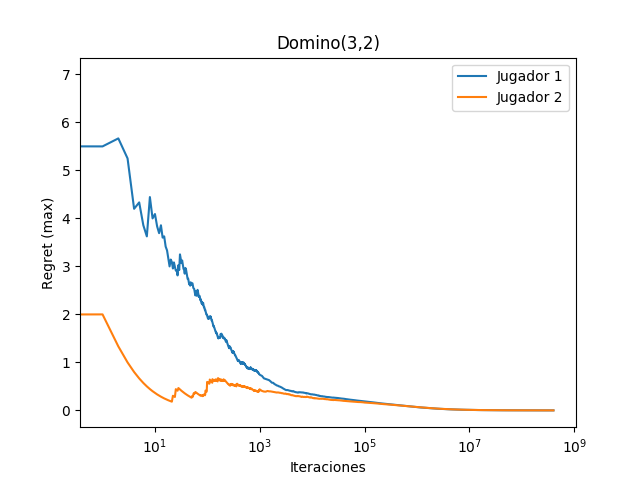
\includegraphics{../graphics/cfr/domino/Domino(3,2).png}}
\end{tabular}}

\resizebox{.9\textwidth}{!}{\begin{tabular}{@{}ccc@{}}
  {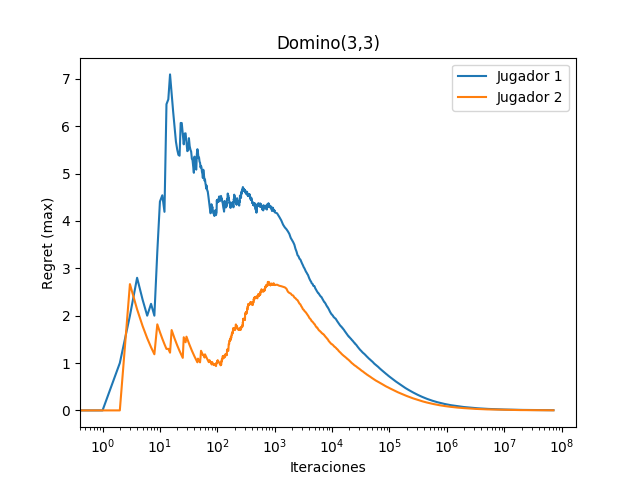
\includegraphics{../graphics/cfr/domino/Domino(3,3).png}} &
  {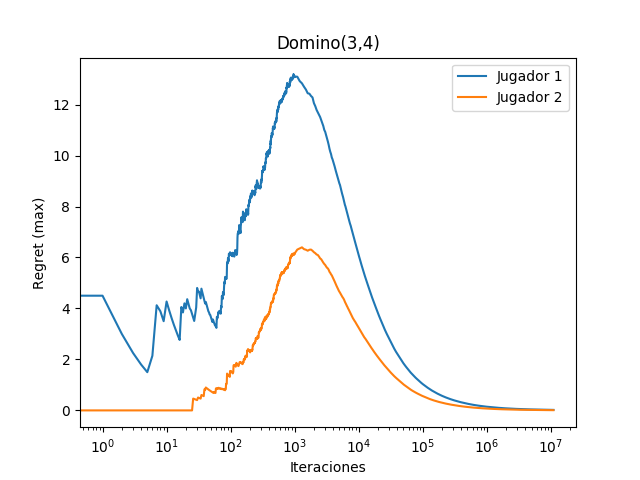
\includegraphics{../graphics/cfr/domino/Domino(3,4).png}}
\end{tabular}}
\end{center}
\end{frame}

\begin{frame}{\Large Experimentos Adicionales}
\begin{enumerate}[--]
  \item Juegos no resueltos con $10$ horas de entrenamiento.
  \item $200$ horas de entrenamiento.
\end{enumerate}

\vspace{.5cm}
\visible<2-3>{%
\Alert{Tabla de Resultados}
\begin{center}
\resizebox{.95\textwidth}{!}{\begin{tabular}{lrrrrrc}
    \toprule
    Juego & $N$ & $I$ & Iteraciones & $u(\sigma)$ & $\varepsilon_{\sigma}$ (\%) & Resuelto \\ \midrule
    \onslide<2>{Dudo$(4, 2, 2)$ &    13.107.101 &      327.680 &    2.276.259 &  0,00875 & 0,2382 & \cmark} \\
    Dudo$(5, 2, 2)$ &                   471.858.976 &    7.864.320 &      133.863 & -0,00004 & 1,7695 & \xmark  \\
    \onslide<2>{Dudo$(6, 1, 2)$ &    66.060.163 &    1.769.472 &      543.485 &   -0,597 & 0,5102 & \cmark} \\
    \onslide<2>{Dudo$(6, 2, 1)$ &    66.060.163 &    1.769.472 &      513.786 &    0,597 & 0,6727 & \cmark} \\
    \onslide<2>{Domino$(3, 4)$  & 1.547.645.185 &      104.050 &  365.484.932 &   3.2027 & 0,1812 & \cmark} \\
    \bottomrule
\end{tabular}}
\end{center}}
\end{frame}

\begin{frame}{\Large Experimentos Adicionales}
\begin{center}
\resizebox{.67\textwidth}{!}{\begin{tabular}{@{}ccc@{}}
  {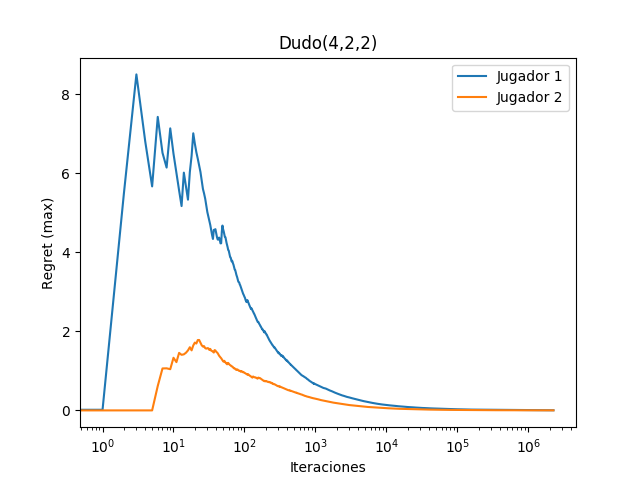
\includegraphics{../graphics/cfr/big_instances/Dudo(4,2,2).png}} &
  {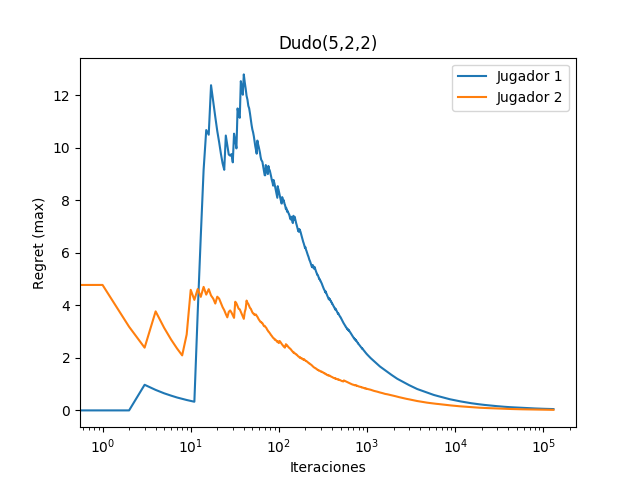
\includegraphics{../graphics/cfr/big_instances/Dudo(5,2,2).png}}
\end{tabular}}
\vspace{.5cm}

\resizebox{\textwidth}{!}{\begin{tabular}{@{}ccc@{}}
  {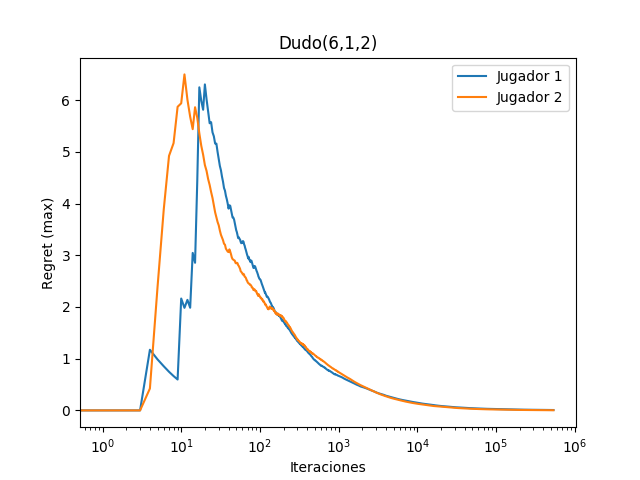
\includegraphics{../graphics/cfr/big_instances/Dudo(6,1,2).png}} &
  {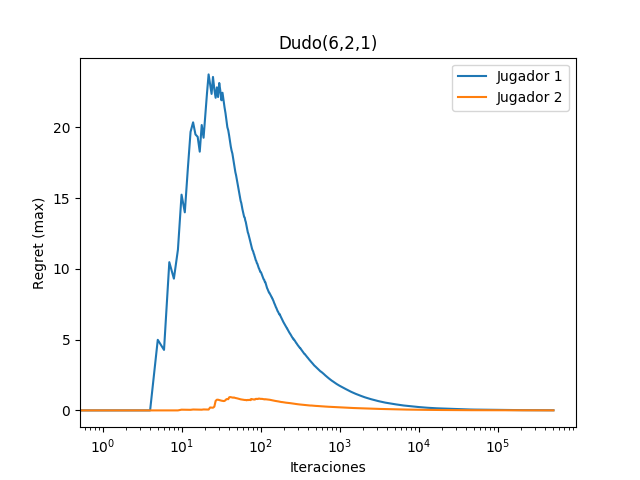
\includegraphics{../graphics/cfr/big_instances/Dudo(6,2,1).png}} &
  {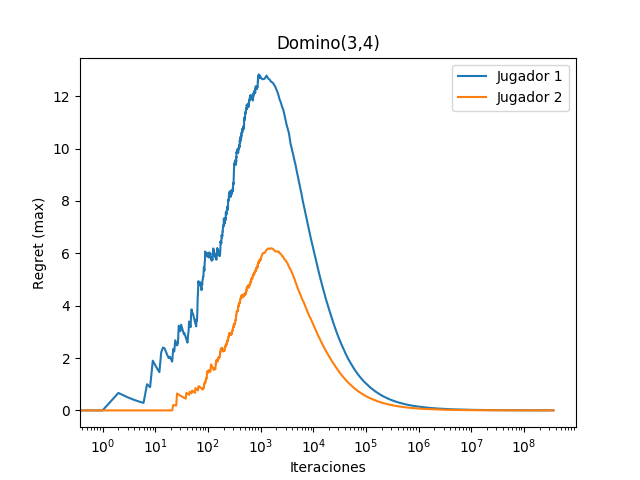
\includegraphics{../graphics/cfr/big_instances/Domino(3,4).png}}
\end{tabular}}
\end{center}
\end{frame}

\begin{frame}{\Large CFR: Conclusiones}
\begin{enumerate}
  \item La forma extesiva es un modelo adecuado para representar juegos secuenciales con informaci\'on incompleta y no determinismo.
  \item El algoritmo CFR permite encontrar un equilibrio de Nash en juegos en forma extensiva de dos jugadores de suma cero.
  \item Se resolvieron diversos juegos captados por el modelos:
  \begin{itemize}
    \item OCP: el segundo tiene ventaja sobre el primer jugador: $u \in (-0.7, -0.5)$.
    \item Dudo: el jugador con mayor n\'umero de dados tiene ventaja.
    \item Domino: el primer jugador tiene ventaja sobre el segundo jugador: $u \in (2, 3.5)$.
  \end{itemize}
\end{enumerate}
\end{frame}

% \begin{frame}{\Large Conclusiones}
% \begin{enumerate}
%   \visible<2->{\item La forma normal y forma extensiva son modelos adecuados para representar juegos con informaci\'on incompleta y no determinista.}
%   \visible<3->{\item El equilibrio de Nash es el principal concepto de soluci\'on utilizado para juegos de dos jugadores de suma cero.}
%   \visible<4->{\item Los algoritmos de Regret Matching y Counterfactual Regret Minimization son efectivos para encontrar una aproximaci\'on a un equilibrio de Nash en el tipo de juego mencionado.}
%   \visible<5->{\item Se utiliz\'o la explotabilidad como m\'etrica para medir la distancia entre una estrategia y un equilibrio de Nash.}
%   \visible<6->{\item Se resolvieron diversos juegos captados por el modelo, incluyendo una versi\'on del juego de domin\'o.}
% \end{enumerate}
% \end{frame}

\begin{frame}{\Large Conclusiones y Recomendaciones}
\Alert{Conclusiones}
\begin{enumerate}
  \item Los modelos utilizados son adecuados para los juegos planteados.
  \item El equilibrio de Nash es un concepto de soluci\'on satisfactorio en juegos de dos jugadores de suma cero. No lo es cuando el juego no es de suma cero o tiene m\'as de dos jugadores.
  \item Se utiliz\'o la explotabilidad como m\'etrica para medir la distancia entre la estrategia obtenida y un equilibrio de Nash.
  \item Resoluci\'on de juegos: se encontraron aproximaciones con una explotabilidad no mayor que el $1\%$ de la m\'inima ganancia positiva posible.
\end{enumerate}

\visible<2->{\Alert{Recomendaciones}}
\begin{enumerate}
  \visible<2->{\item Resolver instancias mayores del juego de domin\'o para $2$ personas considerando abstracciones.}
  \visible<2->{\item Experimentos sobre el juego para $4$ personas considerando cada pareja como un \'unico jugador.}
\end{enumerate}
\end{frame}

\begin{frame}
  \centering{\resizebox{!}{.5cm}{\Alert{Demo}}}
\end{frame}

\begin{frame}
\includemedia[
  width=\textwidth,
  height=.77\textwidth,
  activate=pageopen,
  passcontext,
  transparent,
  addresource=../video/demo,
  flashvars={source=../video/demo}
]{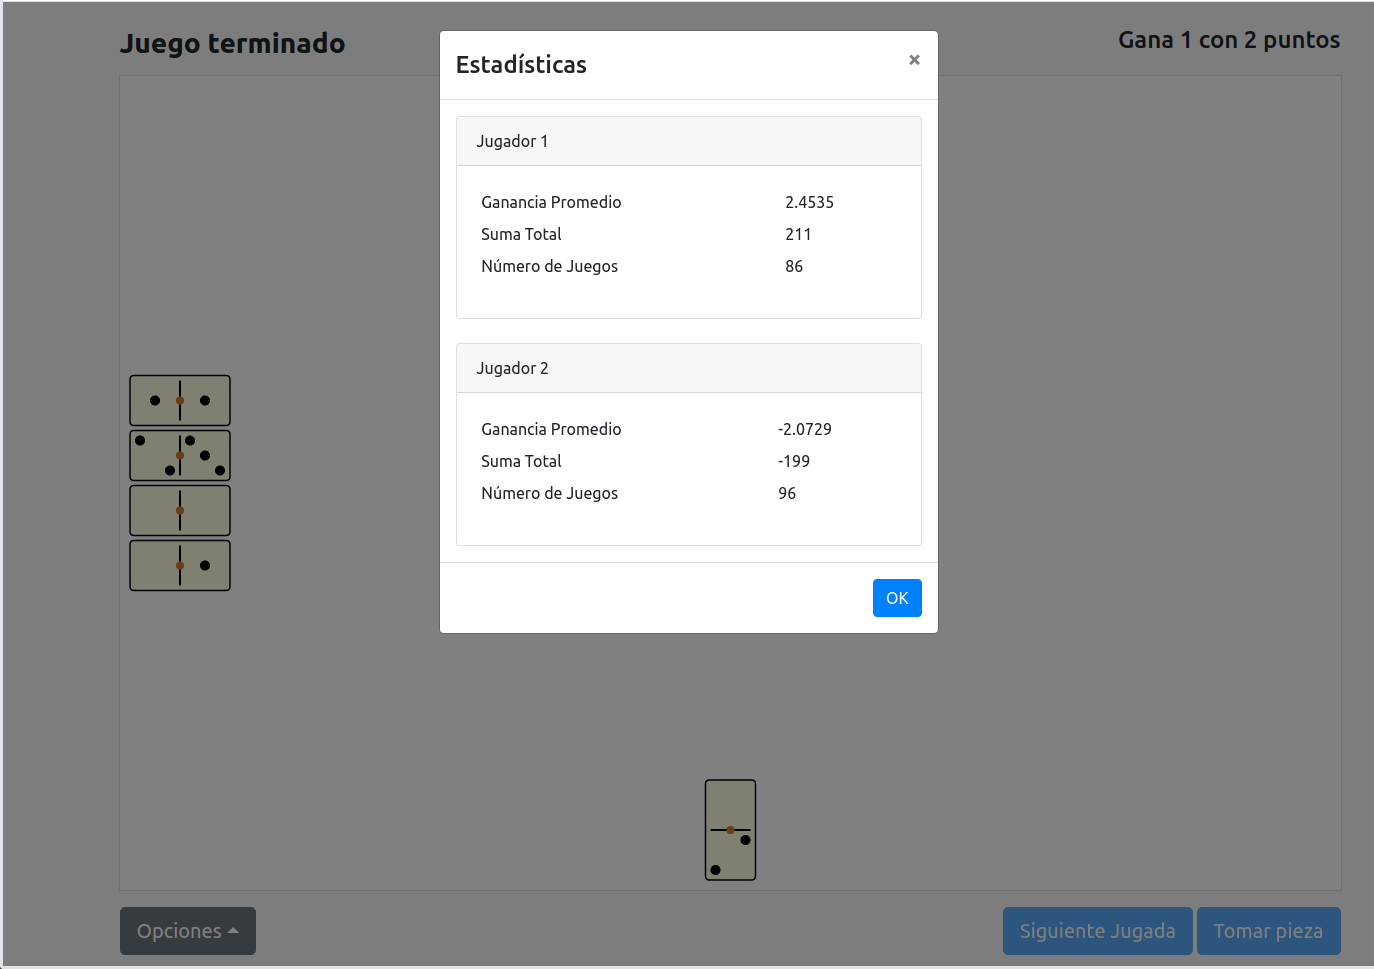
\includegraphics[width=\textwidth]{../video/estadisticas.png}}{VPlayer.swf}
\end{frame}

\begin{frame}
  \centering{\resizebox{!}{.5cm}{\Alert{Gracias por}}}
  \vspace{.1cm}

  \centering{\resizebox{!}{.5cm}{\Alert{su atenci\'on}}}
\end{frame}

\begin{frame}
  \centering{\resizebox{!}{.5cm}{\Alert{?`Preguntas?}}}
\end{frame}

\begin{frame}
  \centering{\resizebox{!}{.5cm}{\Alert{Anexos}}}
\end{frame}

\begin{frame}{\Large Dilema del prisionero.}

(Albert W. Tucker, 1950) Dos prisionerso son sospechosos de un crimen y se interrogan en celdas separadas.
\begin{enumerate}[--]
  \item Si los dos sospechosos se acusan entre entre s\'i ambos reciben una pena de 9 a\~nos de prisi\'on.
  \item Si ninguno acusa al otro, la sentencia ser\'a de 1 a~no de prisi\'on.
  \item Si uno de ellos acusa al otro y el otro no lo hace, quien acus\'o queda en libertad y el otro prisionero es condenado a 15 a\~nos de prisi\'on.
\end{enumerate}

\begin{center}
\begin{tabular}{ c | c | c |}
 \multicolumn{1}{c}{} & \multicolumn{1}{c}{Acusar} & \multicolumn{1}{c}{No Acusar}  \\ \cline{2-3}
 Acusar  &  $-1,-1$ & $-15,0$ \\ \cline{2-3}
 No Acusar    &  $0,-15$ & $-9,-9$ \\ \cline{2-3}
\end{tabular}
\end{center}

\vspace{.2cm}
\RedAlert{Si el juego no es de suma cero, el equilibrio de Nash no es un concepto de soluci\'on satisfactorio.}
\end{frame}

\begin{frame}{\Large Ejemplo de Juego con 3 Jugadores}
\begin{center} \resizebox{.75\textwidth}{!}{\begin{tikzpicture}[
player1/.style={circle, fill=blue, thick, minimum size = 4mm},
player2/.style={circle, fill=red, thick, minimum size=4mm},
player3/.style={circle, fill=ao, thick, minimum size=4mm},
terminal/.style={rectangle, draw=black, fill=black, thick, minimum size=2mm},
level 1/.style={sibling distance=55mm, level distance=25mm},
level 2/.style={sibling distance=27.5mm, level distance=25mm},
level 3/.style={sibling distance=27.5mm, level distance=25mm},
]

\node[player1] {}
  child { node (A) [player2] {}
    child { node[player3] {}
      child { node[terminal] [label=below:{$\left(1, -\frac{1}{2}, -\frac{1}{2}\right)$}] {}
        edge from parent node[left] {$l$}
      }
      child { node[terminal] [label=below:{$\left(-\frac{1}{2}, 1, -\frac{1}{2}\right)$}] {}
        edge from parent node[right] {$r$}
      }
      edge from parent node[left] {$a$}
    }
    child { node[terminal] [label=below:{$(-1, -1, 2)$}] {}
      edge from parent node[right] {$b$}
    }
    edge from parent node[left] [label=above:{$A$}] {}
  }
  child { node (B) [player2] {}
    child {  node[terminal] [label=below:{$(-1, -1, 2)$}] {}
      edge from parent node[left] {$a$}
    }
    child { node [player3] {}
      child { node[terminal] [label=below:{$\left(1, -\frac{1}{2}, -\frac{1}{2}\right)$}] {}
        edge from parent node[left] {$l$}
      }
      child { node[terminal] [label=below:{$\left(-\frac{1}{2}, 1, -\frac{1}{2}\right)$}] {}
        edge from parent node[right] {$r$}
      }
      edge from parent node[right] {$b$}
    }
    edge from parent node[right] [label=above:{$B$}] {}
  }
;
\draw[dashed] (A.east)--(B.west);
\end{tikzpicture}} \end{center}
\begin{enumerate}[--]
\item Los jugadores $1$ y $2$ maximizan su ganancia cuando cooperan.
\item Cuando los jugadores $1$ y $2$ eligen la misma acci\'on el tercer jugador siempre pierde, pero su decisi\'on afecta las ganancias de los otros $2$ jugadores.
\end{enumerate}
\end{frame}

\begin{frame}{Aplicaciones: Seguro de desempleo}
(Rasmusen, 2000) Suponga un individuo. \'El est\'a desempleado y seguir\'a sin buscar empleo mientras el gobierno le ayude a mantener su estilo de vida. El gobierno tratar\'a de darle una ayuda de forma que el individuo est\'e incentivado a buscar un empleo.

\vspace{.25cm}
\begin{center}
\begin{tabular}{ c | c | c |}
 \multicolumn{1}{c}{} & \multicolumn{1}{c}{Buscar Trabajo} & \multicolumn{1}{c}{Descansar}  \\ \cline{2-3}
 Ayudar    &  $5,4$ & $-3,5$ \\ \cline{2-3}
 No Ayudar &  $-3,3$ & $0,0$ \\ \cline{2-3}
\end{tabular}
\end{center}
\end{frame}

\begin{frame}{Aplicaciones: Monopolio Natural}
En este juego existen dos empresas que participan en un monopolio natural. Es decir, el mercado no es lo suficientemente grande para soportar dos empresas. Cada una de las empresas tiene la opci\'on de salir o permanecer en el mercado.

\vspace{.25cm}
\begin{center}
\begin{tabular}{ c | c | c |}
 \multicolumn{1}{c}{} & \multicolumn{1}{c}{Salir} & \multicolumn{1}{c}{Permanecer}  \\ \cline{2-3}
 Salir      & \quad \quad $0,0$ \quad \quad & $0,4$ \\ \cline{2-3}
 Permanecer & \quad \quad $4,0$ \quad \quad & $-2,-2$ \\ \cline{2-3}
\end{tabular}
\end{center}
\end{frame}

\begin{frame}{\Large Perfect Recall}
\begin{enumerate}
  \item El jugador recuerda lo que sab\'ia.
  \item El jugador recuerda lo que eligi\'o.
\end{enumerate}
\begin{center}
\resizebox{.65\textwidth}{!}{\begin{tikzpicture}[
chance/.style={circle, fill=gray, thick, minimum size = 4mm},
player1/.style={circle, fill=blue, thick, minimum size = 4mm},
player2/.style={circle, fill=red, thick, minimum size=4mm},
terminal/.style={rectangle, draw=black, fill=black, thick, minimum size=2mm},
level 1/.style={sibling distance=60mm, level distance=30mm},
level 2/.style={sibling distance=30mm, level distance=25mm},
level 3/.style={sibling distance=30mm, level distance=25mm},
]

\node[chance] [label = {Nodo de azar}] {}
  child { node[player1] [label=above:{A}] {}
    child { node[terminal] [label=below:{$1$}] {}
      edge from parent node[left] {P}
    }
    child { node (A) [player1] [label=above:{B}] {}
      child { node[terminal] [label=below:{$2$}] {}
        edge from parent node[left] {M}
      }
      child { node[terminal] [label=below:{$0$}] {}
        edge from parent node[right] {I}
      }
      edge from parent node[right] {C}
    }
    edge from parent node[left] [label=above:{$2, 1\ \ $}] {}
  }
  child { node[player2] [label=above:{Z}] {}
    child { node (C) [terminal] [label=below:{$-1$}] {}
      edge from parent node[left] {P}
    }
    child { node (B) [player1] [label=above:{B}] {}
      child { node[terminal] [label=below:{$-2$}] {}
        edge from parent node[left] {M}
      }
      child { node[terminal] [label=below:{$0$}] {}
        edge from parent node[right] {I}
      }
      edge from parent node[right] {C}
    }
    edge from parent node[right] [label=above:{$\ \ 1, 2$}] {}
  }
;
\draw[dashed] (A.east) .. controls ++(135:-18mm) and ++(45:-18mm) .. (B.west);
\end{tikzpicture}}
\end{center}
\end{frame}

\begin{frame}{\Large Explotabilidad}
\vspace{.5cm}

\Alert{\only<1-4>{Equilibrio de Nash $\sigma^* = (\sigma^*_1, \sigma^*_2)$}\only<5->{Aproximaci\'on $\sigma' = (\sigma'_1, \sigma'_2)$}}
\visible<2-4, 6->{%
\begin{enumerate}
  \visible<2-4, 6->{\item Primer jugador garantiza una ganancia esperada de \\ al menos \only<2-4>{$u$}\only<6->{$u-\varepsilon_1$}.}
  \visible<3-4, 8->{\item Segundo jugador garantiza una ganancia esperada de \\ \only<3>{al menos $-u$}\only<4, 8->{a lo sumo }\only<4>{$u$}\only<8->{$u+\varepsilon_2$}\only<4, 8->{ para el primer jugador}.\visible<0>{fixheight}}
\end{enumerate}}


\begin{center}
  \begin{tikzpicture}
  \visible<1->{\draw[<->, very thick] (-5.25, 0) -- (5.25, 0);}
  \visible<1->{\draw[dashed] (0, 1.5) -- (0, -1);}
  \visible<1->{\node[align=center] at (0.15, 0.2) {\small{$u$}};}
  \visible<1->{\draw[fill=black] (0, 0) circle (0.05cm);}
  \visible<2>{\draw[->, rounded corners, blue, very thick](0, 0) -- (0, -0.6) -- (5.25, -0.6);}
  \visible<2->{\draw[->, rounded corners, blue, very thin](0, 0) -- (0, -0.6) -- (5.25, -0.6);}
  \visible<2->{\node[text width=3.5cm] at (3.5,-1) {$u_1(\sigma_1^*, \sigma_2) \geq u $};}
  \only<3>{\node[text width=3.5cm] at (-3,-1) {$u_2(\sigma_1, \sigma^*_2) \geq -u $};}
  \visible<3->{\draw[->, rounded corners, red, very thin](0, 0) -- (0, -0.5) -- (-5.25, -0.5);}
  \visible<3-4>{\draw[->, rounded corners, red,  very thick](0, 0) -- (0, -0.5) -- (-5.25, -0.5);}
  \visible<4->{\node[text width=3.5cm] at (-3,-1) {$u_1(\sigma_1, \sigma^*_2) \leq u $};}
  \visible<6->{\draw[<->](-0.01, 1) -- (-1.5, 1);}
  \visible<6->{\draw[dashed] (-1.5, 2) -- (-1.5, -0.45);}
  \visible<6->{\node[text width=1cm] at (-0.4, 1.25) {$\varepsilon_1$};}
  \visible<6->{\node[align=left] at (-0.9, 0.2) {\small{$u-\varepsilon_1$}};}
  \visible<6->{\draw[fill=black] (-1.5, 0) circle (0.05cm);}
  \visible<7->{\draw[->, rounded corners, blue, very thin](-1.5, 0) -- (-1.5, 0.6) -- (5.25, 0.6);}
  \visible<7>{\draw[->, rounded corners, blue, very thick](-1.5, 0) -- (-1.5, 0.6) -- ( 5.25, 0.6);}
  \visible<7->{\node[text width=3.5cm] at (3.5, 1) {$u_1(\sigma'_1, \sigma_2) \geq u - \varepsilon_1$};}
  \visible<8->{\draw[<->](0.01, 1) -- (0.8, 1);}
  \visible<8->{\draw[dashed] (0.8, 2) -- (0.8, -0.45);}
  \visible<8->{\node[text width=1cm] at (0.7, 1.25) {$\varepsilon_2$};}
  \visible<8->{\node[align=left] at (1.35, 0.2) {\small{$u+\varepsilon_2$}};}
  \visible<8->{\draw[fill=black] (0.8, 0) circle (0.05cm);}
  \visible<9->{\draw[->, rounded corners, red, very thin](0.8, 0) -- (0.8, 0.5) -- (-5.25, 0.5);}
  \visible<9>{\draw[->, rounded corners, red,  very thick]( 0.8, 0) -- ( 0.8, 0.5) -- (-5.25, 0.5);}
  \visible<9->{\node[text width=3.5cm] at (-3.25, 1) {$u_1(\sigma_1, \sigma'_2) \leq u + \varepsilon_2$};}
  \visible<10->{\draw[<->](-1.5, 1.7) -- (0.8, 1.7);}
  \visible<10->{\node[text width=1cm] at (0.1, 2) {$\varepsilon$};}
  \end{tikzpicture}

\visible<10->{\Alert{{\Large \textbf{$\varepsilon = \varepsilon_1 + \varepsilon_2$}}}}
\end{center}
\end{frame}

\begin{frame}
  \centering{\resizebox{!}{.5cm}{\Alert{Definiciones y Teoremas}}}
\end{frame}

\begin{frame}[allowframebreaks]{Juegos en Forma Normal o Estrat\'egica}
\begin{block}{Definici\'on}
\label{def:forma-normal}
Un juego de N personas en \textbf{forma normal} (o estrat\'egica) es una tupla $\Gamma = (N, (S_i)_{i \in N}, (u_i)_{i \in N})$, donde:
  \begin{itemize}[]
    \item $N = \{1, 2, \dots, N\}$ es el conjunto de jugadores.
    \item  $S_i$ es el conjunto de \textbf{estrategias puras} (o acciones) del jugador $i$.
    \item $u_i : \Pi _{i \in N} S_i \rightarrow \mathbb{R}$ es la \textbf{funci\'on de pago} del jugador $i$.
  \end{itemize}
\end{block}

\begin{block}{Definici\'on}
Un \textbf{perfil estrat\'egico} (o perfil de acci\'on) es una $N$-tupla formada por una estrategia pura para cada jugador. $S = \Pi_{i \in N}S_i$ es el conjunto de perfiles estrat\'egicos y $s = (s_i)_{i \in N}$ representa un elemento gen\'erico de $S$.
\end{block}

\begin{block}{Definici\'on}
Una \textbf{estrategia mixta} del jugador $i$, denotada con $\sigma_i$, es una distribuci\'on de probabilidad sobre el conjunto $S_i$; es decir $\sigma_i \in \Delta(S_i)$. Se denota con $\sigma_i(s_i)$ la probabilidad de que el jugador $i$ elija la acci\'on $s_i \in S_i$.
\end{block}

\begin{block}{Definici\'on}
El \textbf{soporte} (support) de una estrategia mixta $\sigma_i \in \Delta(S_i)$ del jugador $i$ es el conjunto de estrategias puras con una probabilidad positiva de ser elegidas:
$$\text{support}(\sigma_i)\ =\ \{s_i : \sigma_i(s_i) > 0 \} \,.$$
\end{block}

\begin{block}{Definici\'on}
Un \textbf{perfil estrat\'egico mixto} $\sigma$ consiste en una estrategia mixta para cada jugador; es decir, $\sigma \in \Pi_{i \in N} \Delta(S_i)$ es una tupla de forma $\sigma=(\sigma_i)_{i \in N}$.
\end{block}

\begin{block}{Definici\'on}
La \textbf{ganancia esperada} del jugador $i$ dado un perfil estrat\'egico mixto $\sigma$ es
\begin{align*}
u_i(\sigma)\ =\ \sum_{s \in S} u_i(s) \sigma(s) = \sum_{s \in S} u_i(s) \prod _{j \in N} \sigma_j(s_j) \\ =\ \sum_{s \in S} u_i(s) \sigma_i(s_i) \sigma_{-i}(s_{-i})\,.
\end{align*}
\end{block}

\begin{block}{Teorema}
La ganancia esperada $u_i(\sigma)$ del jugador $i$ dado el perfil estrat\'egico $\sigma$ satisface:
\begin{align*}
u_i(\sigma)\ =\ \sum_{s_i\in S_i} \sigma_i(s_i) \sum_{s_{-i}\in S_{-i}} \sigma_{-i}(s_{-i}) u_i(s_i,s_{-i}) \,.
\end{align*}
\end{block}

\begin{block}{Definici\'on}
Sea $i\in N$ un jugador, $\sigma_i$ una estrategia mixta para el jugador $i$, y $\sigma_{-i}$ un perfil estrat\'egico mixto para el resto de los jugadores. Se dice que $\sigma_i$ es una \textbf{mejor respuesta} con respecto a $\sigma_{-i}$ si y s\'olo si $u_i(\sigma_i,\sigma_{-i}) \geq u_i(\sigma'_i,\sigma_{-i})$ para toda estrategia mixta $\sigma'_i$ para el jugador $i$.
\end{block}

\begin{block}{Definici\'on}
Sea $\sigma^*_i$ una estrategia mixta para el jugador $i$ que es mejor respuesta a $\sigma_{-i}$. Cualquier estrategia mixta $\sigma_i$ para el jugador $i$ cuyo soporte sea un subconjunto del soporte de $\sigma^*_i$ es tambi\'en una mejor respuesta a $\sigma_{-i}$.
\end{block}

\begin{block}{Definici\'on}
Un perfil estrat\'egico mixto $\sigma$ es un \textbf{equilibrio de Nash} si y s\'olo si para todo jugador $i$, la estrategia $\sigma_i$ es mejor respuesta del jugador $i$ para $\sigma_{-i}$.
\end{block}

\begin{block}{Teorema}
Todo juego finito tiene al menos un equilibrio de Nash.
\end{block}

\begin{block}{Definici\'on}
Una distribuci\'on $\psi\in\Delta(S)$ es un \textbf{equilibrio correlacionado} si y s\'olo si para cualquier jugador $i$, y para cualesquiera estrategias puras $x, y \in S_i$,
$$ \sum_{s_{-i}\in S_{-i}} \psi(x,s_{-i}) [ u_i(x,s_{-i}) - u_i(y,s_{-i})]\ \geq\ 0 \,. $$
\end{block}

\begin{block}{Teorema}
Si $\sigma$ es un equilibrio de Nash, entonces $\sigma$ es un equilibrio correlacionado.
\end{block}

\begin{block}{Teorema}
Sea $\psi\in\Delta(S)$ un equilibrio correlacionado. Si $\psi$ se factoriza como $\psi=\prod_{i\in N} \sigma_i$ donde $\{\sigma_i\}_{i\in N}$ es un conjunto de estrategias mixtas para cada jugador (i.e., $\psi(s)=\prod_{i \in N} \sigma_i(s_i)$ para todo $s\in S$), entonces $\psi$ es un equilibrio de Nash.
\end{block}

\begin{block}{Teorema}
Sean $\sigma$ y $\sigma'$ dos equilibrios correlacionados, y $\alpha$ un n\'umero real en $(0,1)$. Entonces, la distribuci\'on $\alpha\sigma + (1-\alpha)\sigma'$ es un equilibrio correlacionado.
\end{block}
\end{frame}

\begin{frame}[allowframebreaks]{Juegos en Forma Extesiva}

\begin{block}{Definici\'on I}
Un juego finito en \textbf{forma extensiva} con \textbf{informaci\'on incompleta} tiene los siguientes componentes:
\begin{itemize}
  \item Un conjunto finito $N$ de \textbf{jugadores}.
  \item Un conjunto finito $H$ de secuencias, las posible \textbf{historias} de acciones, tal que la secuencia vac\'ia est\'a en $H$, y cada prefijo de una secuencia en $H$ tambi\'en est\'a en $H$. $Z \subseteq H$ son las historias terminales (aquellas que no son prefijo de ninguna otra secuencia). $A(h) = \{ a : (h, a) \in H \}$ son las acciones disponibles despu\'es de una historia no terminal $h \in H$. Si la historia $h$ es prefijo de la historia $h'$ escribimos $h\sqsubseteq h'$, y si $h$ es un prefijo propio de $h'$ escribimos $h\sqsubset h'$.
\end{itemize}
\end{block}
\begin{block}{Definici\'on II}
\begin{itemize}
  \item Una funci\'on $P$ que asigna a cada historia no terminal (cada elemento de $H \setminus Z)$ un elemento de $N \cup \{c \}$. $P$ es la \textbf{funci\'on de jugador}. $P(h)$ es el jugador que toma una acci\'on despu\'es de la historia $h$. Si $P(h) = c$ entonces la acci\'on tomada despu\'es de la historia $h$ es determinada por el azar. Este tipo de nodos ser\'an denominados \textbf{nodos de azar}.
  \item Una funci\'on $f_c$ que asocia con cada historia $h$, para la cual $P(h) = c$, una medida de probabilidad $f_c(\cdot|h)$ sobre $A(h)$: $f_c(a|h)$ es la probabilidad de que la acci\'on $a$ ocurra dado $h$. Cada medida de probabilidad es independiente de cualquier otra de estas medidas.
\end{itemize}
\end{block}
\begin{block}{Definici\'on III}
\begin{itemize}
  \item Para cada jugador $i \in N$, una partici\'on $\mathcal{I}_i$ de $\{h \in H : P(h) = i\}$ con la propiedad de que $A(h) = A(h')$ siempre que $h$ y $h'$ est\'en en el mismo bloque de la partici\'on. Para $I_i \in \mathcal{I}_i$ se denota por $A(I_i)$ el conjunto $A(h)$ y por $P(I_i)$ el jugador $P(h)$ para cualquier $h \in I_i$. $\mathcal{I}_i$ es la \textbf{partici\'on de informaci\'on} del jugador $i$, un conjunto $I_i \in \mathcal{I}_i$ es un \textbf{conjunto de informaci\'on} del jugador $i$.
  \item Para cada jugador $i \in N$, una funci\'on de utilidad $u_i$ de los estados terminales $Z$ a los reales $\mathbb{R}$. Si $N = \{1,2\}$ y $u_1 = -u_2$, se dice que se tiene un \textbf{juego de dos jugadores de suma cero en forma extensiva}. Se define $\Delta_{u,i} = \max_z u_i(z) - \min_z u_i(z)$ como el rango de utilidades del jugador $i$.
\end{itemize}
\end{block}

\begin{block}{Definici\'on}
Una \textbf{estrategia pura} para el jugador $i$ es una funci\'on $s_i : \mathcal{I}_i \rightarrow \bigcup_{I_i \in \mathcal{I}_i}A(I_i)$ tal que $s_i(I_i) \in A(I_i)$, donde $A(I_i) = A(h)$ para cualquier $h \in I_i$ es el conjunto de acciones permitidas despu\'es de la historia $h$.
\end{block}

\begin{block}{Definici\'on}
Una \textbf{estrategia mixta} $\sigma^m_i$ para el jugador $i$ es una distribuci\'on de probabilidad sobre $S_i$. Es decir, $\sigma_i^m \in \Delta(S_i)$.
\end{block}

\begin{block}{Definici\'on}
Un \textbf{perfil estrat\'egico mixto} $\sigma^m \in \prod_{i \in N} \Delta(S_i)$ consiste en una estrategia mixta para cada jugador de forma $\sigma^m = (\sigma_1^m, \sigma_2^m, ...., \sigma_N^m)$.
\end{block}

\begin{block}{Definici\'on}
Una \textbf{estrategia de comportamiento} para el jugador $i$ consiste en una distribuci\'on de probabilidad para cada conjunto de informaci\'on $I_i \in \mathcal{I}_i$ sobre el conjunto de acciones $A(I_i)$ que pueden ejecutarse en $I_i$.
Es decir, una estrategia de comportamiento es una tupla $(\sigma^b_i(I_i))_{I_i \in \mathcal{I}_i}$ donde $\sigma^b_i(I_i) \in \Delta(A(I_i))$.
\end{block}

\begin{block}{Definici\'on}
Un \textbf{perfil estrat\'egico de comportamiento} $\sigma^b$ es una estrategia de comportamiento para cada jugador.
\end{block}

\begin{block}{Definici\'on}
Sea $\Sigma=\prod_{i\in N}\Sigma_i$ el conjunto de perfiles mixtos o de comportamiento, seg\'un sea el caso, para los jugadores en $N$ ($\Sigma_i$ es el conjunto de estrategias del jugador $i$).
Para $\varepsilon\geq 0$, se dice que un perfil estrat\'egico $\sigma \in \Sigma$ es un \textbf{$\varepsilon$-equilibrio de Nash} si y s\'olo si para todo jugador $i$ y perfil $\sigma'_i\in\Sigma_i$,
$$ u_i(\sigma) + \varepsilon\ \geq\ u_i(\sigma'_i, \sigma_{-i}) \,. $$
El perfil $\sigma\in\Sigma$ es un \textbf{equilibrio de Nash} si y s\'olo si $\sigma$ es un $0$-equilibrio de Nash.
\end{block}

\begin{block}{Definici\'on}
Se dice que el jugador $i$ tiene \textbf{\textit{perfect recall}} en el juego $\Gamma$ (en forma extensiva) si para cualquier par de historias $h_1, h_2$ con $P(h_1) = P(h_2) = i$, tales que $I(h_1) = I(h_2)$ las siguientes condiciones se cumplen:
\begin{align*}
& h \sqsubseteq h_1\ \implies\ (\exists h' \sqsubseteq h_2 : I(h) = I(h')) \,, \\
& (h_1, a) \sqsubseteq h\  \land\ (h_2, b)\sqsubseteq h'\ \land\ a \neq b\ \  \implies\ I(h) \neq I(h') \,.
\end{align*}
\end{block}

\begin{block}{Definici\'on}
Se dice que dos estrategias $\sigma$ y $\sigma'$ son equivalentes si la probabilidad de alcanzar cualquier historia terminal es la misma; i.e., $\pi^\sigma(z) = \pi^{\sigma'}(z)$ para todo $z \in Z$.
\end{block}

\begin{block}{Definici\'on}
Sea $s_i \in S_i$ una estrategia pura del jugador $i$ e $I_i \in \mathcal{I}$ un conjunto de informaci\'on de dicho jugador. Se dice que $I_i$ es alcanzable bajo $s_i$ si existe una historia $h \in H$ tal que $h \in I_i$ y para toda historia (prefijo) $h' \sqsubset h$ se cumple que: si $P(h') = i$, entonces $(h', s_i(I(h')))$ $\sqsubset$ $h$ y si $P(h') = c$ entonces existe una acci\'on $a$ tal que $(h', a) \sqsubset h$ y la probabilidad de elegir la acci\'on $a$ en $h'$ es positiva, i.e., $f_c(a|h') > 0$.
\end{block}

\begin{block}{Teorema}
Si para el jugador $i$ se cumple que $I(h')\neq I(h)$ para cualquier par de historias $h$ y $h'$ tal que $h'\sqsubset h$ y $P(h)=P(h')=i$, entonces para cualquier estrategia de comportamiento $\sigma^b_i \in B^i$ para el jugador $i$, existe una estrategia mixta $\sigma^m_i$ que es \textbf{equivalente} a $\sigma^b_i$. En particular, la estrategia mixta $\sigma^m_i$ viene dada por:
\begin{align*}
\sigma^m_i(s_i)\ :=\ \prod_{I_i \in \mathcal{I}_i} \sigma^b_i(I_i)(s_i(I_i)) \,.
\end{align*}
\end{block}

\begin{block}{Teorema}
Considere un juego finito de $N$ personas. Si el jugador $i$ tiene ``perfect recall",  entonces para cada estrategia mixta $\sigma^m_i \in \Delta(S_i)$ del jugador $i$, existe una estrategia de comportamiento $\sigma^b_i \in B^i$ equivalente a $\sigma^m_i$.
\end{block}

\begin{block}{Teorema}
Considere un juego finito de $N$ personas. Si el jugador $i$ tiene ``perfect recall",  entonces para cada estrategia mixta $\sigma^m_i \in \Delta(S_i)$ del jugador $i$, existe una estrategia de comportamiento $\sigma^b_i \in B^i$ equivalente a $\sigma^m_i$.
\end{block}

\begin{block}{Teorema}
En un juego con \textit{perfect recall}, cualquier estrategia mixta de un agente dado puede ser remplazada por una estrategia de comportamiento equivalente, y cualquier estrategia de comportamiento puede ser remplazada por una estrategia mixta equivalente. Dos estrategias son equivalentes en el sentido en que inducen los mismos resultados de probabilidades, para cualquier perfil estrat\'egico fijo (mixto o de comportamiento) del resto de los agentes.
\end{block}
\end{frame}

\begin{frame}[allowframebreaks]{Explotabilidad}

\begin{block}{Teorema}
Sea $\sigma^* = (\sigma^*_1, \sigma^*_2)$ un equilibrio de Nash de un juego de dos jugadores de suma cero, tal que $u_1(\sigma) = u$. Entonces $u_i(\sigma^*) \leq u_i(\sigma^*_i, \sigma_{-i})$, para cualquier estrategia $\sigma_{-i}$.
\end{block}

\begin{block}{Teorema}
Sean $\sigma = (\sigma_1, \sigma_2)$ y $\sigma' = (\sigma'_1, \sigma'_2)$ equilibrios de Nash en un juego de dos jugadores con suma cero. Entonces $\sigma'' = (\sigma_1, \sigma'_2)$ y $\sigma''' = (\sigma'_1, \sigma_2)$ son tambi\'en equilibrios de Nash. Adem\'as, $u_i(\sigma) = u_i(\sigma') = u_i(\sigma'') = u_i(\sigma''')$, para $i \in \{1, 2\}$.
\end{block}

\begin{block}{Definici\'on}
Sea $\sigma^* = (\sigma^*_1, \sigma^*_2)$ un equilibrio de Nash en un juego de dos jugadores de suma cero. Sea $\sigma = (\sigma_1, \sigma_2)$ una aproximaci\'on a $\sigma^*$. Sean $\sigma^{\prime}_1$ y $\sigma^{\prime}_2$ las mejores respuesta a $\sigma_2$ y $\sigma_1$, respectivamente. Se definen $\varepsilon_1 = u_2(\sigma_1, \sigma^{\prime}_2) - u_2(\sigma^*)$ y $\varepsilon_2 = u_1(\sigma^{\prime}_1, \sigma_2) - u_1(\sigma^*)$. Luego, la explotabilidad de $\sigma$ es igual a $\varepsilon_{\sigma} = \varepsilon_1 + \varepsilon_2$
\end{block}

\begin{block}{Teorema}
Sean $\sigma$ y $\sigma^{\prime}$ las estrategias definidas en la definici\'on anterior. Luego:
$$\varepsilon_{\sigma} =  u_2(\sigma_1, \sigma^{\prime}_2) + u_1(\sigma^{\prime}_1, \sigma_2)$$
\end{block}
\end{frame}

\begin{frame}[allowframebreaks]{Regret Matching}
\Alert{Regret Condicional}

\begin{align*}
  D_i^t(j, k)\ =\ \frac{1}{t} \sum_{\substack{1\leq \tau \leq t \\s^\tau_i = j}} u_i(k, s_{-i}^{\tau}) - u_i(s^{\tau}) \\
  R_i^t(j, k)\ =\ [D_i^t(j, k)]^+\ =\ \max\{0, D_i^t(j, k)\} \\
  \begin{cases}
    p_{t+1}^i(k)\ :=\  \frac{1}{\mu} R_i^t(j, k) & \text{ si $k \neq j$} \\
    p_{t+1}^i(j)\ :=\ 1 - \sum_{k \in S_i, k \neq j} p_{t+1}^i(k) & \text{si $k=j$}
  \end{cases}
\end{align*}

\begin{block}{Teorema}
Si cada jugador juega de acuerdo al procedimiento descrito arriba, entonces la distribuci\'on emp\'rica del juego $z_t$ converge (a.s.) cuando $t \rightarrow \infty$ al conjunto de equilibrios correlacionado del juego $\Gamma$.
\end{block}

\begin{block}{Teorema}
Sea $(s_t)_{t = 1, 2, ...}$ una secuencia de juegos de $\Gamma$.
Entonces, $R_i^t(j, k)$ converge a $0$ para cada $i$ y cada $j, k \in S_i$, con $j \neq k$, si y s\'olo si la secuencia de distribuciones emp\'ricas $z_t$ converge al conjunto de equilibrio correlacionado.
\end{block}

\framebreak
\Alert{Vector Invariante de Probabilidad}

\begin{align*}
  \begin{cases}
    M^i_t(j, k)\ :=\  \frac{1}{\mu} R_i^t(j, k) & \text{ si $k \neq j$} \\
    M^i_t(j, j)\ :=\ 1 - \sum_{k \in S_i, k \neq j} R^t_i(j,k) & \text{si $k=j$}
  \end{cases}
\end{align*}
Considere un vector (fila) invariante de probabilidad $q^i_t$ (dicho vector siempre existe), donde $q^i_t\in \Delta(S_i)$, para la matriz $M^t$. Es decir, $q^i_t$ satisface $q^i_t \times M^i_t = q^i_t$.

\begin{block}{Teoream}
Sea $R_t^i(j, j) = 0$. El vector $q_t^i$, definido previamente, cumple que:
\begin{align*}
\label{eq:proc-B}
q^i_t(j)\sum_{k \in S_i} R^t_i(j,k)\ =\ \sum_{k \in S_i} q_t^i(k)R_i^t(k,j) \,.
\end{align*}
\end{block}

\begin{block}{Teorema}
Supongamos que a cada per\'iodo $t+1$, el jugador $i$ elige las estrategias acorde a un vector de distribuci\'on de probabilidad $q_t^i$ que satisface la ecuaci\'on anterior. Entonces, $R^i_t(j, k)$ converge a cero (a.s.) para todo $j, k \in S_i$ con $j \neq k$.
\end{block}

\framebreak

\Alert{Regret Incondicional}
\begin{block}{Definition}
Un procedimiento adaptativo es \textbf{universalmente consistente} para el jugador $i$ si:
\begin{align*}
  \limsup_{t \rightarrow \infty } \left[ \max_{k \in S_i} \frac{1}{t} \sum_{\tau = 1}^{t} u_i(k, s_{-i}^{\tau}) - \frac{1}{t} \sum_{\tau = 1}^{t} u_i(s_{\tau}) \right]\ \leq\ 0\quad (a. s.) \,.
\end{align*}
\end{block}

\begin{align*}
D_i^t(k)\ =\ \frac{1}{t} \sum_{\tau = 1}^{t} u_i(k, s_{-i}^{\tau}) - u_i(s_{\tau}) \\
R_i^t(k)\ =\ [D_i^t(k)]^+\ =\ \max\{0, D_i^t(k)\}
\end{align*}

\begin{block}{Teorema}
El procedimiento adaptativo definido previamente es universalmente consistente para el jugador $i$.
\end{block}

\begin{block}{Teorema}
En un procedimiento adaptativo de \textit{Regret Matching}, si el \textit{regret} condicional converge a $0$, entonces el procedimiento es universalmente consistente.
\end{block}

\begin{block}{Teorema}
Sea $\Gamma$ un juego de dos jugadores de suma cero y sea $(s^t)_{t=1,2,..., T}$ una secuencia de juegos de $\Gamma$, tales que, para todo $s_i \in S_i$, para todo $i \in {1, 2}$:
\begin{align*}
\frac{1}{T}\sum_{t = 1}^{T}u_i(s_i, s_{-i}^t) - \frac{1}{T} \sum_{t = 1}^T u_i(s^t)\ \leq\ \varepsilon
\end{align*}
para alg\'un $\varepsilon > 0$. Sea $\bar{\sigma}^T = (\bar{\sigma_1}^T, \bar{\sigma_2}^T)$, donde:
\begin{align*}
\bar{\sigma}_i^T(s_i)\ =\ \frac{|\{ t \leq T : s_i^t = s_i\}|}{T} \,,
\end{align*}
es decir, $\bar{\sigma}^T$ es la distribuci\'on emp\'irica de probabilidad, note que $|\{ t \leq T : s_i^t = s_i\}|$ es igual al n\'umero de veces que se eligi\'o $s_i$ hasta el tiempo $T$. Entonces, $\bar{\sigma}^T$ es un $2\varepsilon$-equilibrio de Nash.
\end{block}
\end{frame}

\begin{frame}[allowframebreaks]{Counterfactual Regret Minimization}
\begin{block}{Definici\'on}
Considere $T$ repeticiones de un juego en forma extensiva indexadas en tiempo por $t=1,2,\ldots,T$. Sea $\sigma^t$ el perfil estrat\'egico de comportamiento utilizado por los jugadores a tiempo $t$ (i.e., $\sigma^t$ consiste de una estrategia de comportamiento $\sigma^t_i$ para cada jugador $i$) . El \textbf{regret promedio general} del jugador $i$ a tiempo $T$ es:
\begin{align*}
R_i^T\ =\ \max_{\sigma^*_i \in B_i} \, \frac{1}{T}\, \sum_{t = 1}^T \, u_i(\sigma_i^*, \sigma_{-i}^t) - u_i(\sigma^t)
\end{align*}
donde $B_i$ es el conjunto de estrategias de comportamiento para el jugador $i$.
\end{block}

Se denotar\'a con $\bar{\sigma}_i^{T}$ la estrategia promedio del jugador $i$, i.e, para cada conjunto de informaci\'on $I \in \mathcal{I}_i$ y para cada acci\'on $a \in A(I)$ se define:
\begin{align*}
\bar{\sigma}_i^{T}(I)(a)\ =\ \frac{\sum_{t = 1}^T \pi^{\sigma^t}_i(I)\,\sigma^t(I)(a)}{\sum_{t = 1}^T \pi^{\sigma^t}_i(I)}
\end{align*}

\begin{block}{Teorema}
En un juego de dos jugadores de suma cero si el regret promedio general a tiempo $T$ es menor que $\varepsilon$ entonces $\bar{\sigma}^{T}=(\bar\sigma^T_1,\bar\sigma^T_2)$ es un $2\varepsilon$-equilibrio de Nash.
\end{block}

\begin{block}{Definici\'on}
Sea $\sigma$ un perfil estrat\'egico e $I \in \mathcal{I}_i$ un conjunto de informaci\'on del jugador $i$, la \textbf{utilidad contrafactual} del par $(\sigma,I)$ es la ganancia esperada dado que el conjunto $I$ es alcanzado y todos los jugadores juegan con la estrategia $\sigma$ con excepci\'on del jugador $i$ que juega para alcanzar $I$. Formalmente:
\begin{align*}
u_i(\sigma, I)\ =\ \frac{\sum_{h \in I, z \in Z} \pi^\sigma_{-i}(h)\, \pi^\sigma(h, z)\, u_i(z)}{\pi^\sigma_{-i}(I)}
\end{align*}
donde $Z$ denota el conjunto de historias terminales, $\pi^\sigma_{-i}(h)$ denota la probabilidad de alcanzar $h$ dado que todos los jugadores utilizan $\sigma$ excepto el jugador $i$ que juega para alcanzar $h$, y $\pi^\sigma(h,h')$ denota la probabilidad de ir de la historia $h$ a la historia $h'$ dado el perfil estrat\'egico $\sigma$; i.e., $\pi^\sigma(h,h')=\pi^\sigma(h')/\pi^\sigma(h)$ si $h \sqsubseteq h'$, y $\pi^\sigma(h, h') = 0$ en caso contrario.
\end{block}

\begin{block}{Definici\'on}
El \textbf{regret contrafactual inmediato} es:
\begin{align*}
R_{i, \text{imm}}^T(I)\ =\  \max_{a \in A(I)} \, \frac{1}{T} \, \sum_{t = 1}^T \, \pi^{\sigma^t}_{-i}(I) \biggl[ u_i(\sigma^t|_{I \rightarrow a}, I) - u_i(\sigma^t, I) \biggr]\,.
\end{align*}
\end{block}

\begin{block}{Teorema}
$R_i^T\ \leq\ \sum_{I \in \mathcal{I}_i} R_{i, \text{imm}}^{T, +}(I)$
\end{block}

\framebreak
\Alert{Regret Minimization}

\begin{block}{Definici\'on}
El \textit{regret} promedio de no haber elegido la acci\'on $a \in A$ hasta tiempo $T$, y en su lugar elegir la acci\'on $a'$ con probabilidad $p^t(a')$ para $t=1,2,\ldots,T$, se define como:
\begin{align*}
R^T(a)\ =\ \frac{1}{T} \sum_{t = 1}^T \left[u^t(a) - \sum_{a' \in A}p^t(a')u^t(a')\right] \,.
\end{align*}
\end{block}

\framebreak
Sea $R^{t, +}(a) = \max\{R^t(a), 0\}$, el algoritmo de \textit{Regret Minimization} consiste en utilizar a tiempo $t$ una distribuci\'on de probabilidad $p^t$, definida por:
\begin{align*}
p^t(a)\ =\
\begin{cases}
\frac{R^{t, +}(a)}{\sum_{a' \in A} R^{t, +}(a')}\ & \text{si }\ \sum_{a' \in A} R^{t, +}(a') > 0 \,, \\
\frac{1}{|A|}\ & \text{en otro caso} \,.
\end{cases}
\end{align*}

\begin{block}{Teorema}
Si $|u| = \max_{t \in \{1, 2, ... T\}} \max_{a, a' \in A}\bigl[u^t(a) - u^t(a')\bigr]$, entonces el regret del algoritmo de Regret Minimization est\'a acotado por:
\begin{align*}
\max_{a \in A}\,R^t(a)\ \leq\ |u| \sqrt{\frac{|A|}{T}} \,.
\end{align*}
\end{block}

\framebreak
\Alert{CFR}

Se mantiene para cada conjunto de informaci\'on $I \in \mathcal{I}_i$ y cada acci\'on $a \in A(I)$, la medida de regret:
\begin{align*}
R_i^T(I, a)\ =\ \frac{1}{T} \sum_{t = 1}^T \pi^{\sigma^t}_{-i}(I)\biggl[u_i(\sigma^t|_{I \rightarrow a}, I) - u_i(\sigma^t, I)\biggr]
\end{align*}

Para $R_i^{T, +}(I, a) = \max\{R_i^T(I, a), 0\}$, definimos la estrategia $\sigma^{T+1}_i$ elegida por el jugador $i$ a tiempo $T+1$:
\begin{align*}
\sigma_i^{T+1}(I)(a)\ =\
\begin{cases}
\frac{R_i^{T, +}(I, a)}{\sum_{a' \in A(I)} R_i^{T, +}(I, a')} & \text{si } \sum_{a' \in A(I) R_i^{T, +}(I, a')} > 0 \,, \\
\frac{1}{|A(I)|} & \text{en otro caso.}
\end{cases}
\end{align*}

\framebreak
\begin{block}{Teorema}
Si el jugador $i$ selecciona las acciones de acuerdo a la Ecuaci\'on anterior, entonces $R^T_{i, \text{imm}}(I) \leq \Delta_{u, i} \sqrt{|A_i|/T}$, donde $|A_i| = \max \{ |A(h)| : P(h) = i \}$ es el m\'aximo n\'umero de acciones que el jugador $i$ tiene disponibles en una historia dada y  $\Delta_{u,i} = \max_{z \in Z}u_i(z) - \min_{z \in Z}u_i(z)$ es el rango de las utilidades del jugador $i$. Luego:
\begin{align*}
R_i^T\ \leq\ \sum_{I\in\mathcal{I}_i} R^{T,+}_{i,imm}(I) \
        \leq\ \Delta_{u,i}\,|\mathcal{I}_i|\,\sqrt{\frac{|A_i|}{T}} \,.
\end{align*}
\end{block}

\framebreak
\Alert{Monte Carlo CFR}
\begin{align*}
\tilde{u}_i(\sigma, I | j)\ =\ \sum_{h \in I, z \in Q_j} \frac{\pi^\sigma_{-i}(h)\,\pi^\sigma(h, z)\, u_i(z)}{q(z)\,\pi^\sigma_{-i}(I)} \,.
\end{align*}

\begin{block}{Teorema}
$E_{j \sim q_j} [\tilde{u}_i(\sigma, I | j)]\ =\ u_i(\sigma, I)$.
\end{block}

\end{frame}

\end{document}
